\documentclass[twoside]{book}

% Packages required by doxygen
\usepackage{fixltx2e}
\usepackage{calc}
\usepackage{doxygen}
\usepackage[export]{adjustbox} % also loads graphicx
\usepackage{graphicx}
\usepackage[utf8]{inputenc}
\usepackage{makeidx}
\usepackage{multicol}
\usepackage{multirow}
\PassOptionsToPackage{warn}{textcomp}
\usepackage{textcomp}
\usepackage[nointegrals]{wasysym}
\usepackage[table]{xcolor}

% Font selection
\usepackage[T1]{fontenc}
\usepackage[scaled=.90]{helvet}
\usepackage{courier}
\usepackage{amssymb}
\usepackage{sectsty}
\renewcommand{\familydefault}{\sfdefault}
\allsectionsfont{%
  \fontseries{bc}\selectfont%
  \color{darkgray}%
}
\renewcommand{\DoxyLabelFont}{%
  \fontseries{bc}\selectfont%
  \color{darkgray}%
}
\newcommand{\+}{\discretionary{\mbox{\scriptsize$\hookleftarrow$}}{}{}}

% Page & text layout
\usepackage{geometry}
\geometry{%
  a4paper,%
  top=2.5cm,%
  bottom=2.5cm,%
  left=2.5cm,%
  right=2.5cm%
}
\tolerance=750
\hfuzz=15pt
\hbadness=750
\setlength{\emergencystretch}{15pt}
\setlength{\parindent}{0cm}
\setlength{\parskip}{3ex plus 2ex minus 2ex}
\makeatletter
\renewcommand{\paragraph}{%
  \@startsection{paragraph}{4}{0ex}{-1.0ex}{1.0ex}{%
    \normalfont\normalsize\bfseries\SS@parafont%
  }%
}
\renewcommand{\subparagraph}{%
  \@startsection{subparagraph}{5}{0ex}{-1.0ex}{1.0ex}{%
    \normalfont\normalsize\bfseries\SS@subparafont%
  }%
}
\makeatother

% Headers & footers
\usepackage{fancyhdr}
\pagestyle{fancyplain}
\fancyhead[LE]{\fancyplain{}{\bfseries\thepage}}
\fancyhead[CE]{\fancyplain{}{}}
\fancyhead[RE]{\fancyplain{}{\bfseries\leftmark}}
\fancyhead[LO]{\fancyplain{}{\bfseries\rightmark}}
\fancyhead[CO]{\fancyplain{}{}}
\fancyhead[RO]{\fancyplain{}{\bfseries\thepage}}
\fancyfoot[LE]{\fancyplain{}{}}
\fancyfoot[CE]{\fancyplain{}{}}
\fancyfoot[RE]{\fancyplain{}{\bfseries\scriptsize Generated by Doxygen }}
\fancyfoot[LO]{\fancyplain{}{\bfseries\scriptsize Generated by Doxygen }}
\fancyfoot[CO]{\fancyplain{}{}}
\fancyfoot[RO]{\fancyplain{}{}}
\renewcommand{\footrulewidth}{0.4pt}
\renewcommand{\chaptermark}[1]{%
  \markboth{#1}{}%
}
\renewcommand{\sectionmark}[1]{%
  \markright{\thesection\ #1}%
}

% Indices & bibliography
\usepackage{natbib}
\usepackage[titles]{tocloft}
\setcounter{tocdepth}{3}
\setcounter{secnumdepth}{5}
\makeindex

% Hyperlinks (required, but should be loaded last)
\usepackage{ifpdf}
\ifpdf
  \usepackage[pdftex,pagebackref=true]{hyperref}
\else
  \usepackage[ps2pdf,pagebackref=true]{hyperref}
\fi
\hypersetup{%
  colorlinks=true,%
  linkcolor=blue,%
  citecolor=blue,%
  unicode%
}

% Custom commands
\newcommand{\clearemptydoublepage}{%
  \newpage{\pagestyle{empty}\cleardoublepage}%
}

\usepackage{caption}
\captionsetup{labelsep=space,justification=centering,font={bf},singlelinecheck=off,skip=4pt,position=top}

%===== C O N T E N T S =====

\begin{document}

% Titlepage & ToC
\hypersetup{pageanchor=false,
             bookmarksnumbered=true,
             pdfencoding=unicode
            }
\pagenumbering{roman}
\begin{titlepage}
\vspace*{7cm}
\begin{center}%
{\Large World War Jump }\\
\vspace*{1cm}
{\large Generated by Doxygen 1.8.11}\\
\end{center}
\end{titlepage}
\clearemptydoublepage
\tableofcontents
\clearemptydoublepage
\pagenumbering{arabic}
\hypersetup{pageanchor=true}

%--- Begin generated contents ---
\chapter{Hierarchical Index}
\section{Class Hierarchy}
This inheritance list is sorted roughly, but not completely, alphabetically\+:\begin{DoxyCompactList}
\item \contentsline{section}{Game\+Settings}{\pageref{class_game_settings}}{}
\item Q\+Graphics\+Pixmap\+Item\begin{DoxyCompactList}
\item \contentsline{section}{Back\+Ground}{\pageref{class_back_ground}}{}
\item \contentsline{section}{Terrain}{\pageref{class_terrain}}{}
\item \contentsline{section}{World\+Object}{\pageref{class_world_object}}{}
\begin{DoxyCompactList}
\item \contentsline{section}{Battle\+Unit}{\pageref{class_battle_unit}}{}
\item \contentsline{section}{Projectile}{\pageref{class_projectile}}{}
\end{DoxyCompactList}
\end{DoxyCompactList}
\item Q\+Graphics\+Rect\+Item\begin{DoxyCompactList}
\item \contentsline{section}{Input}{\pageref{class_input}}{}
\end{DoxyCompactList}
\item Q\+Graphics\+Scene\begin{DoxyCompactList}
\item \contentsline{section}{Gameplay\+Interface}{\pageref{class_gameplay_interface}}{}
\end{DoxyCompactList}
\item Q\+Graphics\+View\begin{DoxyCompactList}
\item \contentsline{section}{Game\+Menu}{\pageref{class_game_menu}}{}
\item \contentsline{section}{Game\+World}{\pageref{class_game_world}}{}
\end{DoxyCompactList}
\item Q\+Main\+Window\begin{DoxyCompactList}
\item \contentsline{section}{Main\+Window}{\pageref{class_main_window}}{}
\end{DoxyCompactList}
\item Q\+Object\begin{DoxyCompactList}
\item \contentsline{section}{Input}{\pageref{class_input}}{}
\item \contentsline{section}{Physics\+Calc}{\pageref{class_physics_calc}}{}
\item \contentsline{section}{Sound\+Player}{\pageref{class_sound_player}}{}
\item \contentsline{section}{World\+Object}{\pageref{class_world_object}}{}
\end{DoxyCompactList}
\end{DoxyCompactList}

\chapter{Class Index}
\section{Class List}
Here are the classes, structs, unions and interfaces with brief descriptions\+:\begin{DoxyCompactList}
\item\contentsline{section}{\hyperlink{class_back_ground}{Back\+Ground} \\*The background class covers the empty circle in the hollow circle in game. -\/ Wang }{\pageref{class_back_ground}}{}
\item\contentsline{section}{\hyperlink{class_battle_unit}{Battle\+Unit} \\*Subclass of \hyperlink{class_world_object}{World\+Object} and represents the player\textquotesingle{}s fighting units on the field }{\pageref{class_battle_unit}}{}
\item\contentsline{section}{\hyperlink{class_game_menu}{Game\+Menu} \\*All necessary things for a functional game menu\+: Pages, buttons and images. It also has parameters which save custom options. -\/ Wang }{\pageref{class_game_menu}}{}
\item\contentsline{section}{\hyperlink{class_gameplay_interface}{Gameplay\+Interface} \\*Displays the \hyperlink{class_terrain}{Terrain}, and the players\textquotesingle{} multiple \hyperlink{class_battle_unit}{Battle\+Unit} and \hyperlink{class_projectile}{Projectile} }{\pageref{class_gameplay_interface}}{}
\item\contentsline{section}{\hyperlink{class_game_settings}{Game\+Settings} \\*\hyperlink{class_game_settings}{Game\+Settings} saves the in-\/game setting... -\/ Tomas and Wang }{\pageref{class_game_settings}}{}
\item\contentsline{section}{\hyperlink{class_game_world}{Game\+World} \\*Container class for \hyperlink{class_terrain}{Terrain}, \hyperlink{class_input}{Input} and \hyperlink{class_gameplay_interface}{Gameplay\+Interface}. -\/ Wang and ... who else? }{\pageref{class_game_world}}{}
\item\contentsline{section}{\hyperlink{class_input}{Input} \\*Receives the players\textquotesingle{} key hits }{\pageref{class_input}}{}
\item\contentsline{section}{\hyperlink{class_main_window}{Main\+Window} }{\pageref{class_main_window}}{}
\item\contentsline{section}{\hyperlink{class_physics_calc}{Physics\+Calc} \\*Our own physics calculator engine and the core of the game. -\/\+Can, Tomas, Sebastian }{\pageref{class_physics_calc}}{}
\item\contentsline{section}{\hyperlink{class_projectile}{Projectile} }{\pageref{class_projectile}}{}
\item\contentsline{section}{\hyperlink{class_sound_player}{Sound\+Player} \\*This is our sound system. -\/ Wang and Can }{\pageref{class_sound_player}}{}
\item\contentsline{section}{\hyperlink{class_terrain}{Terrain} \\*\hyperlink{class_terrain}{Terrain}, the playground for our battle units in form of an inner circle. -\/ W\+A\+NG }{\pageref{class_terrain}}{}
\item\contentsline{section}{\hyperlink{class_world_object}{World\+Object} }{\pageref{class_world_object}}{}
\end{DoxyCompactList}

\chapter{Class Documentation}
\hypertarget{class_back_ground}{}\section{Back\+Ground Class Reference}
\label{class_back_ground}\index{Back\+Ground@{Back\+Ground}}


The background class covers the empty circle in the hollow circle in game. -\/ Wang.  




{\ttfamily \#include $<$background.\+h$>$}

Inheritance diagram for Back\+Ground\+:\begin{figure}[H]
\begin{center}
\leavevmode
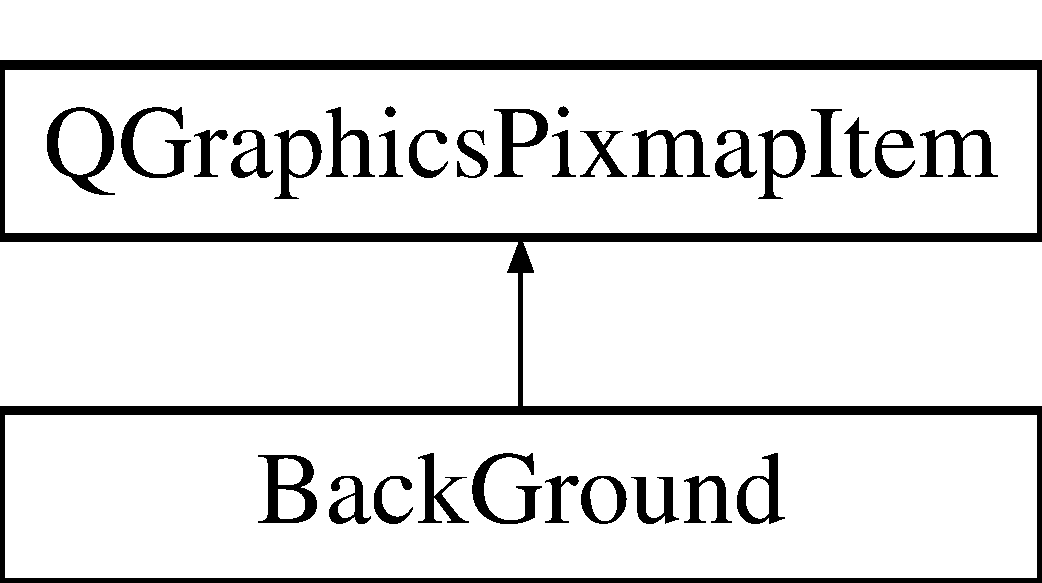
\includegraphics[height=2.000000cm]{class_back_ground}
\end{center}
\end{figure}
\subsection*{Public Member Functions}
\begin{DoxyCompactItemize}
\item 
{\bfseries Back\+Ground} (\hyperlink{class_game_settings}{Game\+Settings} $\ast$settings, Q\+Timer $\ast$back\+Ground\+Rotation\+Timer)\hypertarget{class_back_ground_a30f171b979fa95cff7e4beea65da174e}{}\label{class_back_ground_a30f171b979fa95cff7e4beea65da174e}

\end{DoxyCompactItemize}


\subsection{Detailed Description}
The background class covers the empty circle in the hollow circle in game. -\/ Wang. 

The documentation for this class was generated from the following files\+:\begin{DoxyCompactItemize}
\item 
background.\+h\item 
background.\+cpp\end{DoxyCompactItemize}

\hypertarget{class_battle_unit}{}\section{Battle\+Unit Class Reference}
\label{class_battle_unit}\index{Battle\+Unit@{Battle\+Unit}}


The \hyperlink{class_battle_unit}{Battle\+Unit} class is a subclass of \hyperlink{class_world_object}{World\+Object} and represents the player\textquotesingle{}s fighting units on the field.  




{\ttfamily \#include $<$battleunit.\+h$>$}

Inheritance diagram for Battle\+Unit\+:\begin{figure}[H]
\begin{center}
\leavevmode
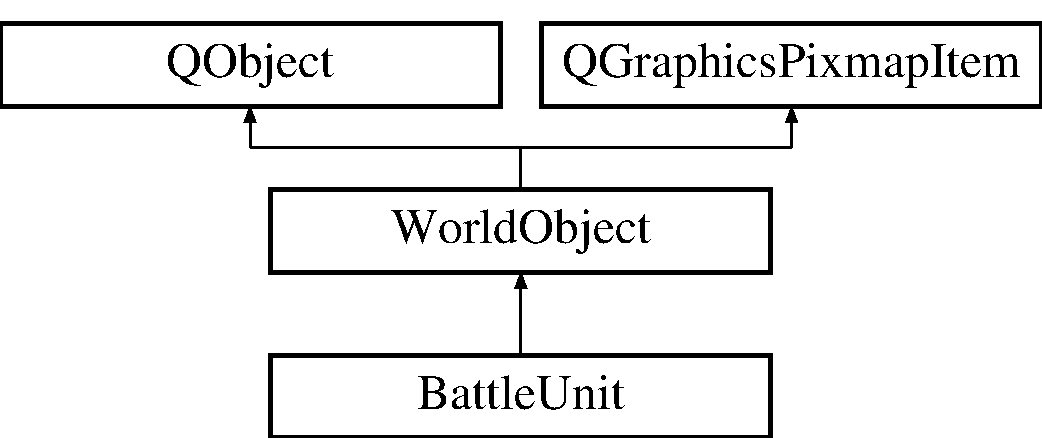
\includegraphics[height=3.000000cm]{class_battle_unit}
\end{center}
\end{figure}
\subsection*{Public Slots}
\begin{DoxyCompactItemize}
\item 
void \hyperlink{class_battle_unit_ad483aca2f0e52cb79c5b0444f6fbd1da}{shoot} ()\hypertarget{class_battle_unit_ad483aca2f0e52cb79c5b0444f6fbd1da}{}\label{class_battle_unit_ad483aca2f0e52cb79c5b0444f6fbd1da}

\begin{DoxyCompactList}\small\item\em \hyperlink{class_battle_unit_ad483aca2f0e52cb79c5b0444f6fbd1da}{Battle\+Unit\+::shoot} spawns projectile when the connected button is pressed. The unit chooses the projectile to choose based on how many times it has been shot before and plays corresponding sound. The Projectile\+Type is cycled and will changed if the instance of the \hyperlink{class_battle_unit}{Battle\+Unit} has hit an enemy. \end{DoxyCompactList}\item 
void {\bfseries set\+Shoot\+Able} ()\hypertarget{class_battle_unit_a32aaaf8056f9545f231a9bdc368aef8f}{}\label{class_battle_unit_a32aaaf8056f9545f231a9bdc368aef8f}

\end{DoxyCompactItemize}
\subsection*{Public Member Functions}
\begin{DoxyCompactItemize}
\item 
\hyperlink{class_battle_unit_ab89fc2d2730cc059c34bb7cd3473d2f0}{Battle\+Unit} (\hyperlink{class_game_world}{Game\+World} $\ast$parent\+View, Player player, \hyperlink{class_sound_player}{Sound\+Player} $\ast$soundplayer, unit\+Type unittype)
\begin{DoxyCompactList}\small\item\em \hyperlink{class_battle_unit_ab89fc2d2730cc059c34bb7cd3473d2f0}{Battle\+Unit\+::\+Battle\+Unit} constructor. Initializes the center of mass dependent on unit type, initializes the unit parameters and connects the jump and shoot signals with respective slots. \end{DoxyCompactList}\item 
double \hyperlink{class_battle_unit_aa5a7ea370e2f789b51f5617b45822bdb}{get\+Firedirection} ()
\begin{DoxyCompactList}\small\item\em \hyperlink{class_battle_unit_aa5a7ea370e2f789b51f5617b45822bdb}{Battle\+Unit\+::get\+Firedirection} returns the fire direction of a battleunit. \end{DoxyCompactList}\item 
void \hyperlink{class_battle_unit_ab038bbc9e82cea88af5a9228c0559463}{set\+Firedirection} (double direction)
\begin{DoxyCompactList}\small\item\em \hyperlink{class_battle_unit_ab038bbc9e82cea88af5a9228c0559463}{Battle\+Unit\+::set\+Firedirection} sets the fire direction of a battleunit. \end{DoxyCompactList}\item 
unit\+Type {\bfseries get\+Unittype} ()\hypertarget{class_battle_unit_a26e22880479bf89c7cc3cec7c8f84a0b}{}\label{class_battle_unit_a26e22880479bf89c7cc3cec7c8f84a0b}

\item 
void \hyperlink{class_battle_unit_a065ad7ba4c947aafd266b7a9e4c523a4}{calculate\+Shooting\+Point} (double $\ast$Point)
\begin{DoxyCompactList}\small\item\em \hyperlink{class_battle_unit_a065ad7ba4c947aafd266b7a9e4c523a4}{Battle\+Unit\+::calculate\+Shooting\+Point} calculate the point where the projectile spawns in scene coordinates. \end{DoxyCompactList}\end{DoxyCompactItemize}
\subsection*{Public Attributes}
\begin{DoxyCompactItemize}
\item 
\hyperlink{class_sound_player}{Sound\+Player} $\ast$ {\bfseries soundpointer}\hypertarget{class_battle_unit_ac450e1e80608c8031e27406bc0be5a90}{}\label{class_battle_unit_ac450e1e80608c8031e27406bc0be5a90}

\end{DoxyCompactItemize}
\subsection*{Additional Inherited Members}


\subsection{Detailed Description}
The \hyperlink{class_battle_unit}{Battle\+Unit} class is a subclass of \hyperlink{class_world_object}{World\+Object} and represents the player\textquotesingle{}s fighting units on the field. 

\subsection{Constructor \& Destructor Documentation}
\index{Battle\+Unit@{Battle\+Unit}!Battle\+Unit@{Battle\+Unit}}
\index{Battle\+Unit@{Battle\+Unit}!Battle\+Unit@{Battle\+Unit}}
\subsubsection[{\texorpdfstring{Battle\+Unit(\+Game\+World $\ast$parent\+View, Player player, Sound\+Player $\ast$soundplayer, unit\+Type unittype)}{BattleUnit(GameWorld *parentView, Player player, SoundPlayer *soundplayer, unitType unittype)}}]{\setlength{\rightskip}{0pt plus 5cm}Battle\+Unit\+::\+Battle\+Unit (
\begin{DoxyParamCaption}
\item[{{\bf Game\+World} $\ast$}]{parent\+View, }
\item[{Player}]{player, }
\item[{{\bf Sound\+Player} $\ast$}]{soundplayer, }
\item[{unit\+Type}]{unittype}
\end{DoxyParamCaption}
)}\hypertarget{class_battle_unit_ab89fc2d2730cc059c34bb7cd3473d2f0}{}\label{class_battle_unit_ab89fc2d2730cc059c34bb7cd3473d2f0}


\hyperlink{class_battle_unit_ab89fc2d2730cc059c34bb7cd3473d2f0}{Battle\+Unit\+::\+Battle\+Unit} constructor. Initializes the center of mass dependent on unit type, initializes the unit parameters and connects the jump and shoot signals with respective slots. 


\begin{DoxyParams}{Parameters}
{\em parent\+View} & pointer to connect() the \hyperlink{class_battle_unit}{Battle\+Unit} to the player\textquotesingle{}s input and the game\textquotesingle{}s refresh rate. \\
\hline
{\em player} & the player controlling the unit \\
\hline
{\em soundplayer} & the pointer to the global sound player \\
\hline
{\em unittype} & the enum that gives the battle unit type\\
\hline
\end{DoxyParams}
The \hyperlink{class_battle_unit}{Battle\+Unit} is only allowed to shoot every certain milliseconds, set in \hyperlink{class_game_settings}{Game\+Settings}. 

\subsection{Member Function Documentation}
\index{Battle\+Unit@{Battle\+Unit}!calculate\+Shooting\+Point@{calculate\+Shooting\+Point}}
\index{calculate\+Shooting\+Point@{calculate\+Shooting\+Point}!Battle\+Unit@{Battle\+Unit}}
\subsubsection[{\texorpdfstring{calculate\+Shooting\+Point(double $\ast$\+Point)}{calculateShootingPoint(double *Point)}}]{\setlength{\rightskip}{0pt plus 5cm}void Battle\+Unit\+::calculate\+Shooting\+Point (
\begin{DoxyParamCaption}
\item[{double $\ast$}]{Point}
\end{DoxyParamCaption}
)}\hypertarget{class_battle_unit_a065ad7ba4c947aafd266b7a9e4c523a4}{}\label{class_battle_unit_a065ad7ba4c947aafd266b7a9e4c523a4}


\hyperlink{class_battle_unit_a065ad7ba4c947aafd266b7a9e4c523a4}{Battle\+Unit\+::calculate\+Shooting\+Point} calculate the point where the projectile spawns in scene coordinates. 


\begin{DoxyParams}{Parameters}
{\em Point} & the array to be changed into shooting point \\
\hline
\end{DoxyParams}
\index{Battle\+Unit@{Battle\+Unit}!get\+Firedirection@{get\+Firedirection}}
\index{get\+Firedirection@{get\+Firedirection}!Battle\+Unit@{Battle\+Unit}}
\subsubsection[{\texorpdfstring{get\+Firedirection()}{getFiredirection()}}]{\setlength{\rightskip}{0pt plus 5cm}double Battle\+Unit\+::get\+Firedirection (
\begin{DoxyParamCaption}
{}
\end{DoxyParamCaption}
)}\hypertarget{class_battle_unit_aa5a7ea370e2f789b51f5617b45822bdb}{}\label{class_battle_unit_aa5a7ea370e2f789b51f5617b45822bdb}


\hyperlink{class_battle_unit_aa5a7ea370e2f789b51f5617b45822bdb}{Battle\+Unit\+::get\+Firedirection} returns the fire direction of a battleunit. 

\begin{DoxyReturn}{Returns}
return the fire direction in angles 
\end{DoxyReturn}
\index{Battle\+Unit@{Battle\+Unit}!set\+Firedirection@{set\+Firedirection}}
\index{set\+Firedirection@{set\+Firedirection}!Battle\+Unit@{Battle\+Unit}}
\subsubsection[{\texorpdfstring{set\+Firedirection(double direction)}{setFiredirection(double direction)}}]{\setlength{\rightskip}{0pt plus 5cm}void Battle\+Unit\+::set\+Firedirection (
\begin{DoxyParamCaption}
\item[{double}]{direction}
\end{DoxyParamCaption}
)}\hypertarget{class_battle_unit_ab038bbc9e82cea88af5a9228c0559463}{}\label{class_battle_unit_ab038bbc9e82cea88af5a9228c0559463}


\hyperlink{class_battle_unit_ab038bbc9e82cea88af5a9228c0559463}{Battle\+Unit\+::set\+Firedirection} sets the fire direction of a battleunit. 


\begin{DoxyParams}{Parameters}
{\em direction} & the fire direction in angles \\
\hline
\end{DoxyParams}


The documentation for this class was generated from the following files\+:\begin{DoxyCompactItemize}
\item 
World\+War\+Jump/\+World\+War\+Jump/battleunit.\+h\item 
World\+War\+Jump/\+World\+War\+Jump/battleunit.\+cpp\end{DoxyCompactItemize}

\hypertarget{class_game_menu}{}\section{Game\+Menu Class Reference}
\label{class_game_menu}\index{Game\+Menu@{Game\+Menu}}


The \hyperlink{class_game_menu}{Game\+Menu} class contains all necessary things for a functional game menu\+: Pages, buttons and images. It also has parameters which save custom options. -\/ Wang.  




{\ttfamily \#include $<$gamemenu.\+h$>$}

Inheritance diagram for Game\+Menu\+:\begin{figure}[H]
\begin{center}
\leavevmode
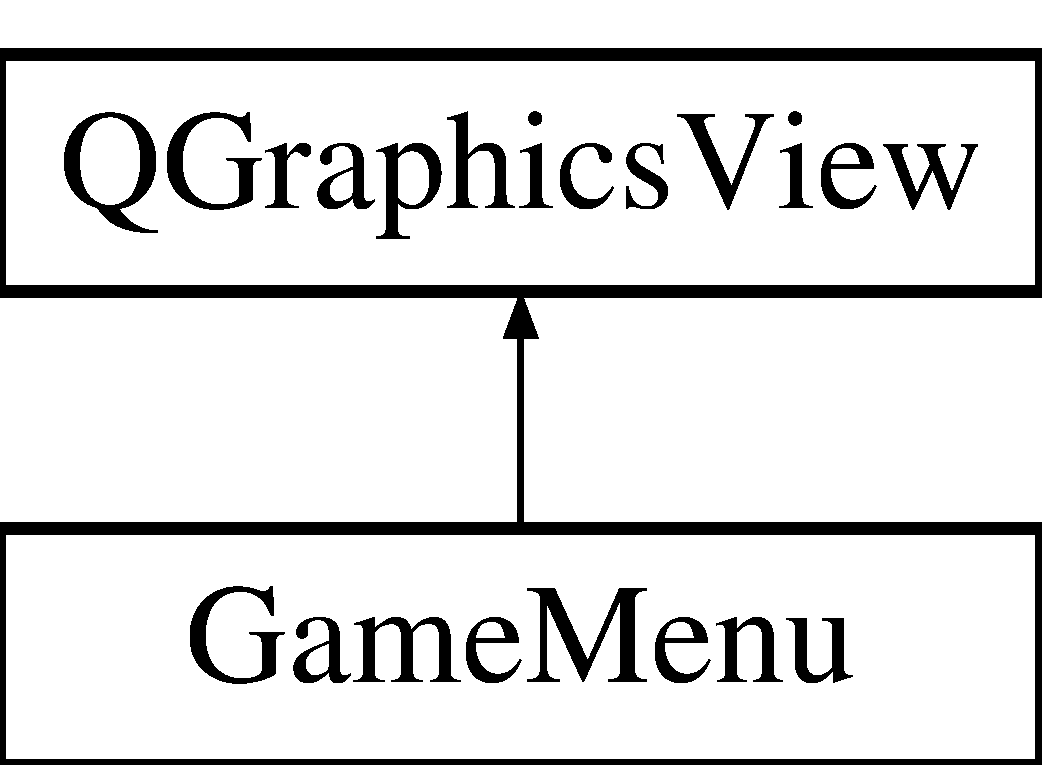
\includegraphics[height=2.000000cm]{class_game_menu}
\end{center}
\end{figure}
\subsection*{Public Slots}
\begin{DoxyCompactItemize}
\item 
void \hyperlink{class_game_menu_a3e3677db66b2c65a9f0de92f41fe3698}{playeronewon} ()\hypertarget{class_game_menu_a3e3677db66b2c65a9f0de92f41fe3698}{}\label{class_game_menu_a3e3677db66b2c65a9f0de92f41fe3698}

\begin{DoxyCompactList}\small\item\em \hyperlink{class_game_menu_a3e3677db66b2c65a9f0de92f41fe3698}{Game\+Menu\+::playeronewon()} triggers once the physics calculator says the game is over and player red has won. It shows the end-\/game scene, then deletes the game scene with it\textquotesingle{}s children. \end{DoxyCompactList}\item 
void \hyperlink{class_game_menu_a7cf2904dfdb06e5bd6423d80fda61739}{playertwowon} ()\hypertarget{class_game_menu_a7cf2904dfdb06e5bd6423d80fda61739}{}\label{class_game_menu_a7cf2904dfdb06e5bd6423d80fda61739}

\begin{DoxyCompactList}\small\item\em \hyperlink{class_game_menu_a7cf2904dfdb06e5bd6423d80fda61739}{Game\+Menu\+::playertwowon()} triggers once the physics calculator says the game is over and player blue has won. It shows the end-\/game scene, then deletes the game scene with it\textquotesingle{}s children. \end{DoxyCompactList}\item 
void \hyperlink{class_game_menu_a41521364226c92bfdedc97b4445c8763}{change\+B\+G\+Mvolume} (int volume)
\begin{DoxyCompactList}\small\item\em \hyperlink{class_game_menu_a41521364226c92bfdedc97b4445c8763}{Game\+Menu\+::change\+B\+G\+Mvolume(int volume)} sets the volume of the background music to the given number. \end{DoxyCompactList}\item 
void \hyperlink{class_game_menu_abb166085ca8e741d1901cdedda86f0d3}{change\+S\+Evolume} (int volume)
\begin{DoxyCompactList}\small\item\em \hyperlink{class_game_menu_abb166085ca8e741d1901cdedda86f0d3}{Game\+Menu\+::change\+S\+Evolume(int volume)} sets the volume of sound effects to the given number. \end{DoxyCompactList}\end{DoxyCompactItemize}
\subsection*{Public Member Functions}
\begin{DoxyCompactItemize}
\item 
\hyperlink{class_game_menu_acc7215518fa676e7985aa3f34ca55ef7}{Game\+Menu} (\hyperlink{class_sound_player}{Sound\+Player} $\ast$soundplayer)
\begin{DoxyCompactList}\small\item\em \hyperlink{class_game_menu_acc7215518fa676e7985aa3f34ca55ef7}{Game\+Menu\+::\+Game\+Menu(\+Sound\+Player $\ast$soundplayer)} constructor instantiates the setting of the game, start\+Scene, which is the main menu, and several buttons and pictures. \end{DoxyCompactList}\item 
int \hyperlink{class_game_menu_adc24456c629b662425a461b7171da615}{get\+Game\+Menu\+Size} () const 
\begin{DoxyCompactList}\small\item\em \hyperlink{class_game_menu_adc24456c629b662425a461b7171da615}{Game\+Menu\+::get\+Game\+Menu\+Size()} returns the set resolution of the game menu. \end{DoxyCompactList}\item 
void \hyperlink{class_game_menu_aeb35fbd4176b7069dd59395b39d1950c}{set\+Game\+Menu\+Size} (int value)
\begin{DoxyCompactList}\small\item\em \hyperlink{class_game_menu_aeb35fbd4176b7069dd59395b39d1950c}{Game\+Menu\+::set\+Game\+Menu\+Size(int value)} sets the resolution of the menu. \end{DoxyCompactList}\item 
void \hyperlink{class_game_menu_ab043085d1280afd8f33c5e962a171373}{mouse\+Press\+Event} (Q\+Mouse\+Event $\ast$event)\hypertarget{class_game_menu_ab043085d1280afd8f33c5e962a171373}{}\label{class_game_menu_ab043085d1280afd8f33c5e962a171373}

\begin{DoxyCompactList}\small\item\em \hyperlink{class_game_menu_ab043085d1280afd8f33c5e962a171373}{Game\+Menu\+::mouse\+Press\+Event(\+Q\+Mouse\+Event $\ast$event)} secures the main functionality of the menu. It detects mouse clicks and compares the Q\+Graphics\+Item on which the mouse is currently positioned with buttons, which are inherited from Q\+Graphics\+Pixmap\+Item, then acts correspondingly. \end{DoxyCompactList}\item 
int \hyperlink{class_game_menu_ac37e4932a0aa396be6ffb04cad2061b2}{get\+Player1\+Unit\+Count} () const 
\item 
int \hyperlink{class_game_menu_a9fd03816511faec236d787298237b231}{get\+Player2\+Unit\+Count} () const 
\item 
int \hyperlink{class_game_menu_a45729234e7d5e250608217f0b24ac8da}{get\+Which\+Stage} () const 
\begin{DoxyCompactList}\small\item\em \hyperlink{class_game_menu_a45729234e7d5e250608217f0b24ac8da}{Game\+Menu\+::get\+Which\+Stage()} returns the index of the currently selected stage. \end{DoxyCompactList}\end{DoxyCompactItemize}
\subsection*{Public Attributes}
\begin{DoxyCompactItemize}
\item 
\hyperlink{class_game_settings}{Game\+Settings} $\ast$ {\bfseries settings}\hypertarget{class_game_menu_a0047e42e8cef38e9faa5ba67d6dea508}{}\label{class_game_menu_a0047e42e8cef38e9faa5ba67d6dea508}

\item 
\hyperlink{class_sound_player}{Sound\+Player} $\ast$ \hyperlink{class_game_menu_a9dfd20cecbc58d41918f85f08942065d}{soundpointer}\hypertarget{class_game_menu_a9dfd20cecbc58d41918f85f08942065d}{}\label{class_game_menu_a9dfd20cecbc58d41918f85f08942065d}

\begin{DoxyCompactList}\small\item\em because soundplayer is instantiated in main, we need this as a reference to gain access on it. \end{DoxyCompactList}\item 
\hyperlink{class_game_world}{Game\+World} $\ast$ \hyperlink{class_game_menu_acd0a5b94ff397f9247088d5942c27341}{reference}\hypertarget{class_game_menu_acd0a5b94ff397f9247088d5942c27341}{}\label{class_game_menu_acd0a5b94ff397f9247088d5942c27341}

\begin{DoxyCompactList}\small\item\em used to gain access on created game. \end{DoxyCompactList}\item 
\hyperlink{class_main_window}{Main\+Window} $\ast$ {\bfseries w} = new \hyperlink{class_main_window}{Main\+Window}\hypertarget{class_game_menu_ab2cbc2fb13a1e67c958efe22a58c5ec2}{}\label{class_game_menu_ab2cbc2fb13a1e67c958efe22a58c5ec2}

\item 
Q\+Graphics\+Scene $\ast$ \hyperlink{class_game_menu_ab72c5ce17a0f06580b74c495cb9694ce}{start\+Scene}\hypertarget{class_game_menu_ab72c5ce17a0f06580b74c495cb9694ce}{}\label{class_game_menu_ab72c5ce17a0f06580b74c495cb9694ce}

\begin{DoxyCompactList}\small\item\em is the main menu. \end{DoxyCompactList}\item 
Q\+Graphics\+Scene $\ast$ \hyperlink{class_game_menu_a96efe4b74ad120a5920e141cec544f94}{before\+Game\+Scene}\hypertarget{class_game_menu_a96efe4b74ad120a5920e141cec544f94}{}\label{class_game_menu_a96efe4b74ad120a5920e141cec544f94}

\begin{DoxyCompactList}\small\item\em is the scene between main menu and game scene. \end{DoxyCompactList}\item 
Q\+Graphics\+Scene $\ast$ \hyperlink{class_game_menu_a034da5f5a381412e92d1764f5af32883}{settings\+Scene}\hypertarget{class_game_menu_a034da5f5a381412e92d1764f5af32883}{}\label{class_game_menu_a034da5f5a381412e92d1764f5af32883}

\begin{DoxyCompactList}\small\item\em is the setting menu for sound. \end{DoxyCompactList}\item 
Q\+Graphics\+Scene $\ast$ \hyperlink{class_game_menu_a347306846ed65b9ed5ed3d457e46c5ac}{about\+Scene}\hypertarget{class_game_menu_a347306846ed65b9ed5ed3d457e46c5ac}{}\label{class_game_menu_a347306846ed65b9ed5ed3d457e46c5ac}

\begin{DoxyCompactList}\small\item\em is the about page. \end{DoxyCompactList}\item 
Q\+Graphics\+Scene $\ast$ \hyperlink{class_game_menu_a235b359eff5bab01a8ca9d2b75466af1}{end\+Scene}\hypertarget{class_game_menu_a235b359eff5bab01a8ca9d2b75466af1}{}\label{class_game_menu_a235b359eff5bab01a8ca9d2b75466af1}

\begin{DoxyCompactList}\small\item\em is the scene after someone has won. \end{DoxyCompactList}\item 
Q\+Graphics\+Pixmap\+Item $\ast$ \hyperlink{class_game_menu_ab6fd3496d0426f663e9893a893764fcf}{start\+Scene\+Background}\hypertarget{class_game_menu_ab6fd3496d0426f663e9893a893764fcf}{}\label{class_game_menu_ab6fd3496d0426f663e9893a893764fcf}

\begin{DoxyCompactList}\small\item\em is the background picture for main menu. \end{DoxyCompactList}\item 
Q\+Graphics\+Pixmap\+Item $\ast$ \hyperlink{class_game_menu_a59aa0e84b5d4db53a62bb52480856c25}{before\+Game\+Scene\+Background}\hypertarget{class_game_menu_a59aa0e84b5d4db53a62bb52480856c25}{}\label{class_game_menu_a59aa0e84b5d4db53a62bb52480856c25}

\begin{DoxyCompactList}\small\item\em is the background picture for pregame settings. \end{DoxyCompactList}\item 
Q\+Graphics\+Pixmap\+Item $\ast$ \hyperlink{class_game_menu_a32c0e1b35559b840ffc5628cb59c8639}{end\+Scene\+Background}\hypertarget{class_game_menu_a32c0e1b35559b840ffc5628cb59c8639}{}\label{class_game_menu_a32c0e1b35559b840ffc5628cb59c8639}

\begin{DoxyCompactList}\small\item\em is the background picture for winning scene. \end{DoxyCompactList}\item 
Q\+Graphics\+Pixmap\+Item $\ast$ {\bfseries start\+Button}\hypertarget{class_game_menu_a22c3e73fc24f9699e6a9f4bc1d6fbd52}{}\label{class_game_menu_a22c3e73fc24f9699e6a9f4bc1d6fbd52}

\item 
Q\+Graphics\+Pixmap\+Item $\ast$ {\bfseries settings\+Button}\hypertarget{class_game_menu_aca49d1e3a9dfec037cbc85a01cb6df82}{}\label{class_game_menu_aca49d1e3a9dfec037cbc85a01cb6df82}

\item 
Q\+Graphics\+Pixmap\+Item $\ast$ {\bfseries about\+Button}\hypertarget{class_game_menu_a3d6ca189f02e14ed5cfb5451526a271b}{}\label{class_game_menu_a3d6ca189f02e14ed5cfb5451526a271b}

\item 
Q\+Graphics\+Pixmap\+Item $\ast$ {\bfseries exit\+Button}\hypertarget{class_game_menu_a76bcbc6a772fb628f39140c9365eccd8}{}\label{class_game_menu_a76bcbc6a772fb628f39140c9365eccd8}

\item 
Q\+Graphics\+Pixmap\+Item $\ast$ {\bfseries add\+Player1\+Unit\+Button}\hypertarget{class_game_menu_aedcd8869665d66f9489ab41f0c038df8}{}\label{class_game_menu_aedcd8869665d66f9489ab41f0c038df8}

\item 
Q\+Graphics\+Pixmap\+Item $\ast$ {\bfseries add\+Player2\+Unit\+Button}\hypertarget{class_game_menu_a1027a5d9f67523cee6782d6413a75281}{}\label{class_game_menu_a1027a5d9f67523cee6782d6413a75281}

\item 
Q\+Graphics\+Pixmap\+Item $\ast$ {\bfseries add\+Red\+Tank\+Button}\hypertarget{class_game_menu_aab61d7c4576ad32880dd7ef88ed20ec8}{}\label{class_game_menu_aab61d7c4576ad32880dd7ef88ed20ec8}

\item 
Q\+Graphics\+Pixmap\+Item $\ast$ {\bfseries add\+Red\+Ship\+Button}\hypertarget{class_game_menu_a37bec2390eed30904e9c3a8ba96cc300}{}\label{class_game_menu_a37bec2390eed30904e9c3a8ba96cc300}

\item 
Q\+Graphics\+Pixmap\+Item $\ast$ {\bfseries remove\+Red\+Tank\+Button}\hypertarget{class_game_menu_a27d6aaab28d7b33fe1838a3bfd99d6b4}{}\label{class_game_menu_a27d6aaab28d7b33fe1838a3bfd99d6b4}

\item 
Q\+Graphics\+Pixmap\+Item $\ast$ {\bfseries remove\+Red\+Ship\+Button}\hypertarget{class_game_menu_aa3d84cd45a3fcb796c3f7e558dffdfc7}{}\label{class_game_menu_aa3d84cd45a3fcb796c3f7e558dffdfc7}

\item 
Q\+Graphics\+Pixmap\+Item $\ast$ {\bfseries add\+Blue\+Tank\+Button}\hypertarget{class_game_menu_a3bad751deea1957b875bdbda8543429b}{}\label{class_game_menu_a3bad751deea1957b875bdbda8543429b}

\item 
Q\+Graphics\+Pixmap\+Item $\ast$ {\bfseries add\+Blue\+Ship\+Button}\hypertarget{class_game_menu_a96db625de02a04609bef8a13a663110d}{}\label{class_game_menu_a96db625de02a04609bef8a13a663110d}

\item 
Q\+Graphics\+Pixmap\+Item $\ast$ {\bfseries remove\+Blue\+Tank\+Button}\hypertarget{class_game_menu_ac2e4f8f3a0a760347ce8aae8a3471c48}{}\label{class_game_menu_ac2e4f8f3a0a760347ce8aae8a3471c48}

\item 
Q\+Graphics\+Pixmap\+Item $\ast$ {\bfseries remove\+Blue\+Ship\+Button}\hypertarget{class_game_menu_a5291121c9137f0f5395dc907e0fab7d0}{}\label{class_game_menu_a5291121c9137f0f5395dc907e0fab7d0}

\item 
Q\+Graphics\+Pixmap\+Item $\ast$ {\bfseries remove\+Player1\+Unit\+Button}\hypertarget{class_game_menu_addbd2f8181f964d60fda59124bab548d}{}\label{class_game_menu_addbd2f8181f964d60fda59124bab548d}

\item 
Q\+Graphics\+Pixmap\+Item $\ast$ {\bfseries remove\+Player2\+Unit\+Button}\hypertarget{class_game_menu_ae4e2074109a89d582cb9e88e83f37a36}{}\label{class_game_menu_ae4e2074109a89d582cb9e88e83f37a36}

\item 
Q\+Graphics\+Pixmap\+Item $\ast$ {\bfseries change\+Stage\+Button}\hypertarget{class_game_menu_a7305ba1cbd36a0c0383968581977b66e}{}\label{class_game_menu_a7305ba1cbd36a0c0383968581977b66e}

\item 
Q\+Graphics\+Pixmap\+Item $\ast$ {\bfseries start\+Battle\+Button}\hypertarget{class_game_menu_a63e87ded92f5c386c776fdf0db70c391}{}\label{class_game_menu_a63e87ded92f5c386c776fdf0db70c391}

\item 
Q\+Graphics\+Pixmap\+Item $\ast$ {\bfseries back\+Button}\hypertarget{class_game_menu_a5095d622706253beec6b63056c09e872}{}\label{class_game_menu_a5095d622706253beec6b63056c09e872}

\item 
Q\+Graphics\+Pixmap\+Item $\ast$ {\bfseries friendly\+Fire\+Button}\hypertarget{class_game_menu_acbf50def7da8afa135d24e6a0f8a8a92}{}\label{class_game_menu_acbf50def7da8afa135d24e6a0f8a8a92}

\item 
Q\+Graphics\+Pixmap\+Item $\ast$ {\bfseries yesorno}\hypertarget{class_game_menu_ad650020a1b9c6076803203746289cca3}{}\label{class_game_menu_ad650020a1b9c6076803203746289cca3}

\item 
Q\+Graphics\+Pixmap\+Item $\ast$ {\bfseries player1\+Unit\+Picture}\hypertarget{class_game_menu_a7b6ec049efa3d2edb073b0c6f8d4410c}{}\label{class_game_menu_a7b6ec049efa3d2edb073b0c6f8d4410c}

\item 
Q\+Graphics\+Pixmap\+Item $\ast$ {\bfseries player2\+Unit\+Picture}\hypertarget{class_game_menu_af1854743b63b9756bfd6ce0761918e7e}{}\label{class_game_menu_af1854743b63b9756bfd6ce0761918e7e}

\item 
Q\+Graphics\+Pixmap\+Item $\ast$ {\bfseries stage\+Picture}\hypertarget{class_game_menu_ac9149690e856b17578f3f7fdb932f7a1}{}\label{class_game_menu_ac9149690e856b17578f3f7fdb932f7a1}

\item 
Q\+Graphics\+Pixmap\+Item $\ast$ {\bfseries title\+Picture}\hypertarget{class_game_menu_ad6a103544d02d3cb04f33dfe35676c00}{}\label{class_game_menu_ad6a103544d02d3cb04f33dfe35676c00}

\item 
Q\+Graphics\+Pixmap\+Item $\ast$ {\bfseries player1\+Unit\+Count\+Picture}\hypertarget{class_game_menu_a1fb70748425976821089be584d3f3840}{}\label{class_game_menu_a1fb70748425976821089be584d3f3840}

\item 
Q\+Graphics\+Pixmap\+Item $\ast$ {\bfseries player2\+Unit\+Count\+Picture}\hypertarget{class_game_menu_aa68b9697560092eb9c78d10945df0b1f}{}\label{class_game_menu_aa68b9697560092eb9c78d10945df0b1f}

\item 
Q\+Graphics\+Pixmap\+Item $\ast$ {\bfseries player\+Red\+Ship\+Count\+Picture}\hypertarget{class_game_menu_a930dfe40b7944b923cba0573a1ac2e55}{}\label{class_game_menu_a930dfe40b7944b923cba0573a1ac2e55}

\item 
Q\+Graphics\+Pixmap\+Item $\ast$ {\bfseries player\+Red\+Tank\+Count\+Picture}\hypertarget{class_game_menu_a5e1eaab4a213cf591a8f795170385cec}{}\label{class_game_menu_a5e1eaab4a213cf591a8f795170385cec}

\item 
Q\+Graphics\+Pixmap\+Item $\ast$ {\bfseries player\+Blue\+Ship\+Count\+Picture}\hypertarget{class_game_menu_a7ed3930e5a8f355cd35a71324b83623f}{}\label{class_game_menu_a7ed3930e5a8f355cd35a71324b83623f}

\item 
Q\+Graphics\+Pixmap\+Item $\ast$ {\bfseries player\+Blue\+Tank\+Count\+Picture}\hypertarget{class_game_menu_a29de28479797b06dfe7dd9b45d5f028d}{}\label{class_game_menu_a29de28479797b06dfe7dd9b45d5f028d}

\item 
Q\+Graphics\+Pixmap\+Item $\ast$ {\bfseries red\+Ship\+Picture}\hypertarget{class_game_menu_ae84c38f6ebfb2e3ff1706cbc68486664}{}\label{class_game_menu_ae84c38f6ebfb2e3ff1706cbc68486664}

\item 
Q\+Graphics\+Pixmap\+Item $\ast$ {\bfseries red\+Tank\+Picture}\hypertarget{class_game_menu_a45bc69ba75f458e21d7f3a1ea63dd666}{}\label{class_game_menu_a45bc69ba75f458e21d7f3a1ea63dd666}

\item 
Q\+Graphics\+Pixmap\+Item $\ast$ {\bfseries blue\+Ship\+Picture}\hypertarget{class_game_menu_ad46b5b1b90f4d0ce99790c8bc9d7832c}{}\label{class_game_menu_ad46b5b1b90f4d0ce99790c8bc9d7832c}

\item 
Q\+Graphics\+Pixmap\+Item $\ast$ {\bfseries blue\+Tank\+Picture}\hypertarget{class_game_menu_af70e2733344a7eeb1678c2666e3eb164}{}\label{class_game_menu_af70e2733344a7eeb1678c2666e3eb164}

\item 
Q\+Graphics\+Pixmap\+Item $\ast$ {\bfseries thumbnail}\hypertarget{class_game_menu_ab8ec0b01e303715a988e5e51cccb14de}{}\label{class_game_menu_ab8ec0b01e303715a988e5e51cccb14de}

\item 
Q\+Graphics\+Pixmap\+Item $\ast$ {\bfseries mute\+B\+G\+M\+Button}\hypertarget{class_game_menu_aaf654b46140ebb546578a3fefd72934c}{}\label{class_game_menu_aaf654b46140ebb546578a3fefd72934c}

\item 
Q\+Graphics\+Pixmap\+Item $\ast$ {\bfseries mute\+S\+E\+Button}\hypertarget{class_game_menu_a23666659fe3b9f0642fd53d308e9a8e0}{}\label{class_game_menu_a23666659fe3b9f0642fd53d308e9a8e0}

\item 
Q\+Graphics\+Pixmap\+Item $\ast$ {\bfseries bgm\+Volume}\hypertarget{class_game_menu_a693030c5c46cdb795d89879a2a362cc2}{}\label{class_game_menu_a693030c5c46cdb795d89879a2a362cc2}

\item 
Q\+Graphics\+Pixmap\+Item $\ast$ {\bfseries se\+Volume}\hypertarget{class_game_menu_a321abee561f05b81fb6e6570ce0b3203}{}\label{class_game_menu_a321abee561f05b81fb6e6570ce0b3203}

\item 
Q\+Graphics\+Pixmap\+Item $\ast$ {\bfseries volume\+Hint}\hypertarget{class_game_menu_a7ee482589366f76c2f28b85df5fe834a}{}\label{class_game_menu_a7ee482589366f76c2f28b85df5fe834a}

\item 
Q\+Slider $\ast$ {\bfseries B\+G\+Mslider}\hypertarget{class_game_menu_a2554f0222dad16e6943190265b4a063d}{}\label{class_game_menu_a2554f0222dad16e6943190265b4a063d}

\item 
Q\+Slider $\ast$ {\bfseries S\+Eslider}\hypertarget{class_game_menu_a1571c2f246e226b8fcc1ff927183d178}{}\label{class_game_menu_a1571c2f246e226b8fcc1ff927183d178}

\item 
Q\+Graphics\+Pixmap\+Item $\ast$ {\bfseries settings\+Background}\hypertarget{class_game_menu_a1883be9e761bc6ddf651d076792a6536}{}\label{class_game_menu_a1883be9e761bc6ddf651d076792a6536}

\item 
Q\+Graphics\+Pixmap\+Item $\ast$ {\bfseries about\+Background}\hypertarget{class_game_menu_abef2252ea78c533c26e57aeaa4b7ac75}{}\label{class_game_menu_abef2252ea78c533c26e57aeaa4b7ac75}

\item 
Q\+Graphics\+Pixmap\+Item $\ast$ {\bfseries playeronewins\+Pic}\hypertarget{class_game_menu_a607f26f22eabdc52789ec0fcb9ae1fd8}{}\label{class_game_menu_a607f26f22eabdc52789ec0fcb9ae1fd8}

\item 
Q\+Graphics\+Pixmap\+Item $\ast$ {\bfseries playertwowins\+Pic}\hypertarget{class_game_menu_a0aa1ea5e275d456d9eaaae032cbf798f}{}\label{class_game_menu_a0aa1ea5e275d456d9eaaae032cbf798f}

\end{DoxyCompactItemize}


\subsection{Detailed Description}
The \hyperlink{class_game_menu}{Game\+Menu} class contains all necessary things for a functional game menu\+: Pages, buttons and images. It also has parameters which save custom options. -\/ Wang. 

\subsection{Constructor \& Destructor Documentation}
\index{Game\+Menu@{Game\+Menu}!Game\+Menu@{Game\+Menu}}
\index{Game\+Menu@{Game\+Menu}!Game\+Menu@{Game\+Menu}}
\subsubsection[{\texorpdfstring{Game\+Menu(\+Sound\+Player $\ast$soundplayer)}{GameMenu(SoundPlayer *soundplayer)}}]{\setlength{\rightskip}{0pt plus 5cm}Game\+Menu\+::\+Game\+Menu (
\begin{DoxyParamCaption}
\item[{{\bf Sound\+Player} $\ast$}]{soundplayer}
\end{DoxyParamCaption}
)}\hypertarget{class_game_menu_acc7215518fa676e7985aa3f34ca55ef7}{}\label{class_game_menu_acc7215518fa676e7985aa3f34ca55ef7}


\hyperlink{class_game_menu_acc7215518fa676e7985aa3f34ca55ef7}{Game\+Menu\+::\+Game\+Menu(\+Sound\+Player $\ast$soundplayer)} constructor instantiates the setting of the game, start\+Scene, which is the main menu, and several buttons and pictures. 


\begin{DoxyParams}{Parameters}
{\em soundplayer} & Because the soundplayer is instantiated already in main.\+cpp, we need to pass it from main to \hyperlink{class_game_menu}{Game\+Menu}. \\
\hline
\end{DoxyParams}


\subsection{Member Function Documentation}
\index{Game\+Menu@{Game\+Menu}!change\+B\+G\+Mvolume@{change\+B\+G\+Mvolume}}
\index{change\+B\+G\+Mvolume@{change\+B\+G\+Mvolume}!Game\+Menu@{Game\+Menu}}
\subsubsection[{\texorpdfstring{change\+B\+G\+Mvolume}{changeBGMvolume}}]{\setlength{\rightskip}{0pt plus 5cm}void Game\+Menu\+::change\+B\+G\+Mvolume (
\begin{DoxyParamCaption}
\item[{int}]{volume}
\end{DoxyParamCaption}
)\hspace{0.3cm}{\ttfamily [slot]}}\hypertarget{class_game_menu_a41521364226c92bfdedc97b4445c8763}{}\label{class_game_menu_a41521364226c92bfdedc97b4445c8763}


\hyperlink{class_game_menu_a41521364226c92bfdedc97b4445c8763}{Game\+Menu\+::change\+B\+G\+Mvolume(int volume)} sets the volume of the background music to the given number. 


\begin{DoxyParams}{Parameters}
{\em volume} & wished volume. \\
\hline
\end{DoxyParams}
\index{Game\+Menu@{Game\+Menu}!change\+S\+Evolume@{change\+S\+Evolume}}
\index{change\+S\+Evolume@{change\+S\+Evolume}!Game\+Menu@{Game\+Menu}}
\subsubsection[{\texorpdfstring{change\+S\+Evolume}{changeSEvolume}}]{\setlength{\rightskip}{0pt plus 5cm}void Game\+Menu\+::change\+S\+Evolume (
\begin{DoxyParamCaption}
\item[{int}]{volume}
\end{DoxyParamCaption}
)\hspace{0.3cm}{\ttfamily [slot]}}\hypertarget{class_game_menu_abb166085ca8e741d1901cdedda86f0d3}{}\label{class_game_menu_abb166085ca8e741d1901cdedda86f0d3}


\hyperlink{class_game_menu_abb166085ca8e741d1901cdedda86f0d3}{Game\+Menu\+::change\+S\+Evolume(int volume)} sets the volume of sound effects to the given number. 


\begin{DoxyParams}{Parameters}
{\em volume} & wished volume \\
\hline
\end{DoxyParams}
\index{Game\+Menu@{Game\+Menu}!get\+Game\+Menu\+Size@{get\+Game\+Menu\+Size}}
\index{get\+Game\+Menu\+Size@{get\+Game\+Menu\+Size}!Game\+Menu@{Game\+Menu}}
\subsubsection[{\texorpdfstring{get\+Game\+Menu\+Size() const }{getGameMenuSize() const }}]{\setlength{\rightskip}{0pt plus 5cm}int Game\+Menu\+::get\+Game\+Menu\+Size (
\begin{DoxyParamCaption}
{}
\end{DoxyParamCaption}
) const}\hypertarget{class_game_menu_adc24456c629b662425a461b7171da615}{}\label{class_game_menu_adc24456c629b662425a461b7171da615}


\hyperlink{class_game_menu_adc24456c629b662425a461b7171da615}{Game\+Menu\+::get\+Game\+Menu\+Size()} returns the set resolution of the game menu. 

\begin{DoxyReturn}{Returns}
the set resolution of the menu 
\end{DoxyReturn}
\index{Game\+Menu@{Game\+Menu}!get\+Player1\+Unit\+Count@{get\+Player1\+Unit\+Count}}
\index{get\+Player1\+Unit\+Count@{get\+Player1\+Unit\+Count}!Game\+Menu@{Game\+Menu}}
\subsubsection[{\texorpdfstring{get\+Player1\+Unit\+Count() const }{getPlayer1UnitCount() const }}]{\setlength{\rightskip}{0pt plus 5cm}int Game\+Menu\+::get\+Player1\+Unit\+Count (
\begin{DoxyParamCaption}
{}
\end{DoxyParamCaption}
) const}\hypertarget{class_game_menu_ac37e4932a0aa396be6ffb04cad2061b2}{}\label{class_game_menu_ac37e4932a0aa396be6ffb04cad2061b2}
\hyperlink{class_game_menu_ac37e4932a0aa396be6ffb04cad2061b2}{Game\+Menu\+::get\+Player1\+Unit\+Count()} returns the unit count of player red (redundant). \index{Game\+Menu@{Game\+Menu}!get\+Player2\+Unit\+Count@{get\+Player2\+Unit\+Count}}
\index{get\+Player2\+Unit\+Count@{get\+Player2\+Unit\+Count}!Game\+Menu@{Game\+Menu}}
\subsubsection[{\texorpdfstring{get\+Player2\+Unit\+Count() const }{getPlayer2UnitCount() const }}]{\setlength{\rightskip}{0pt plus 5cm}int Game\+Menu\+::get\+Player2\+Unit\+Count (
\begin{DoxyParamCaption}
{}
\end{DoxyParamCaption}
) const}\hypertarget{class_game_menu_a9fd03816511faec236d787298237b231}{}\label{class_game_menu_a9fd03816511faec236d787298237b231}
\hyperlink{class_game_menu_a9fd03816511faec236d787298237b231}{Game\+Menu\+::get\+Player2\+Unit\+Count()} returns the unit cound of blue player (redundant). \index{Game\+Menu@{Game\+Menu}!get\+Which\+Stage@{get\+Which\+Stage}}
\index{get\+Which\+Stage@{get\+Which\+Stage}!Game\+Menu@{Game\+Menu}}
\subsubsection[{\texorpdfstring{get\+Which\+Stage() const }{getWhichStage() const }}]{\setlength{\rightskip}{0pt plus 5cm}int Game\+Menu\+::get\+Which\+Stage (
\begin{DoxyParamCaption}
{}
\end{DoxyParamCaption}
) const}\hypertarget{class_game_menu_a45729234e7d5e250608217f0b24ac8da}{}\label{class_game_menu_a45729234e7d5e250608217f0b24ac8da}


\hyperlink{class_game_menu_a45729234e7d5e250608217f0b24ac8da}{Game\+Menu\+::get\+Which\+Stage()} returns the index of the currently selected stage. 

\begin{DoxyReturn}{Returns}
index of the current stage. 
\end{DoxyReturn}
\index{Game\+Menu@{Game\+Menu}!set\+Game\+Menu\+Size@{set\+Game\+Menu\+Size}}
\index{set\+Game\+Menu\+Size@{set\+Game\+Menu\+Size}!Game\+Menu@{Game\+Menu}}
\subsubsection[{\texorpdfstring{set\+Game\+Menu\+Size(int value)}{setGameMenuSize(int value)}}]{\setlength{\rightskip}{0pt plus 5cm}void Game\+Menu\+::set\+Game\+Menu\+Size (
\begin{DoxyParamCaption}
\item[{int}]{value}
\end{DoxyParamCaption}
)}\hypertarget{class_game_menu_aeb35fbd4176b7069dd59395b39d1950c}{}\label{class_game_menu_aeb35fbd4176b7069dd59395b39d1950c}


\hyperlink{class_game_menu_aeb35fbd4176b7069dd59395b39d1950c}{Game\+Menu\+::set\+Game\+Menu\+Size(int value)} sets the resolution of the menu. 


\begin{DoxyParams}{Parameters}
{\em value} & is the wished resolution \\
\hline
\end{DoxyParams}


The documentation for this class was generated from the following files\+:\begin{DoxyCompactItemize}
\item 
gamemenu.\+h\item 
gamemenu.\+cpp\end{DoxyCompactItemize}

\hypertarget{class_gameplay_interface}{}\section{Gameplay\+Interface Class Reference}
\label{class_gameplay_interface}\index{Gameplay\+Interface@{Gameplay\+Interface}}


The \hyperlink{class_gameplay_interface}{Gameplay\+Interface} class displays the \hyperlink{class_terrain}{Terrain}, and the players\textquotesingle{} multiple \hyperlink{class_battle_unit}{Battle\+Unit} and \hyperlink{class_projectile}{Projectile}.  




{\ttfamily \#include $<$Gameplay\+Interface.\+h$>$}

Inheritance diagram for Gameplay\+Interface\+:\begin{figure}[H]
\begin{center}
\leavevmode
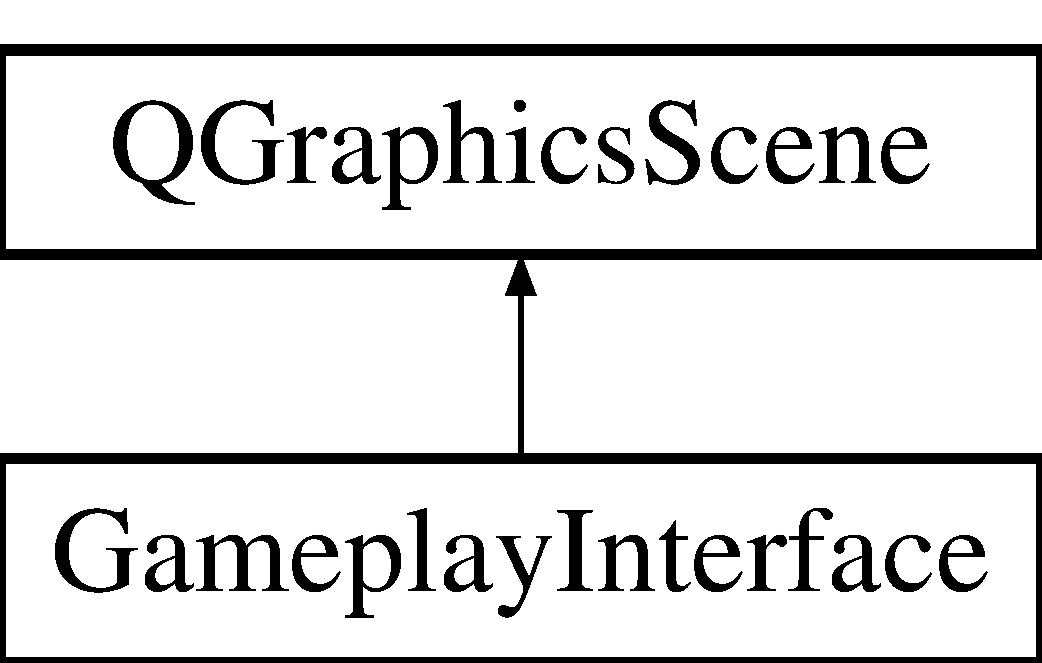
\includegraphics[height=2.000000cm]{class_gameplay_interface}
\end{center}
\end{figure}
\subsection*{Public Member Functions}
\begin{DoxyCompactItemize}
\item 
\hyperlink{class_gameplay_interface_ab75b8894a36f5697edc87e0acc2d31ce}{Gameplay\+Interface} (\hyperlink{class_sound_player}{Sound\+Player} $\ast$soundplayer)
\begin{DoxyCompactList}\small\item\em \hyperlink{class_gameplay_interface_ab75b8894a36f5697edc87e0acc2d31ce}{Gameplay\+Interface\+::\+Gameplay\+Interface}. \end{DoxyCompactList}\end{DoxyCompactItemize}
\subsection*{Public Attributes}
\begin{DoxyCompactItemize}
\item 
\hyperlink{class_physics_calc}{Physics\+Calc} $\ast$ {\bfseries physics\+Calulator}\hypertarget{class_gameplay_interface_adf09add3928dd254e051c3ecc070bee6}{}\label{class_gameplay_interface_adf09add3928dd254e051c3ecc070bee6}

\end{DoxyCompactItemize}


\subsection{Detailed Description}
The \hyperlink{class_gameplay_interface}{Gameplay\+Interface} class displays the \hyperlink{class_terrain}{Terrain}, and the players\textquotesingle{} multiple \hyperlink{class_battle_unit}{Battle\+Unit} and \hyperlink{class_projectile}{Projectile}. 

Furthermore, the \hyperlink{class_gameplay_interface}{Gameplay\+Interface} contains our physical engine \hyperlink{class_physics_calc}{Physics\+Calc}. 

\subsection{Constructor \& Destructor Documentation}
\index{Gameplay\+Interface@{Gameplay\+Interface}!Gameplay\+Interface@{Gameplay\+Interface}}
\index{Gameplay\+Interface@{Gameplay\+Interface}!Gameplay\+Interface@{Gameplay\+Interface}}
\subsubsection[{\texorpdfstring{Gameplay\+Interface(\+Sound\+Player $\ast$soundplayer)}{GameplayInterface(SoundPlayer *soundplayer)}}]{\setlength{\rightskip}{0pt plus 5cm}Gameplay\+Interface\+::\+Gameplay\+Interface (
\begin{DoxyParamCaption}
\item[{{\bf Sound\+Player} $\ast$}]{soundplayer}
\end{DoxyParamCaption}
)}\hypertarget{class_gameplay_interface_ab75b8894a36f5697edc87e0acc2d31ce}{}\label{class_gameplay_interface_ab75b8894a36f5697edc87e0acc2d31ce}


\hyperlink{class_gameplay_interface_ab75b8894a36f5697edc87e0acc2d31ce}{Gameplay\+Interface\+::\+Gameplay\+Interface}. 


\begin{DoxyParams}{Parameters}
{\em soundplayer} & static values for the scene\textquotesingle{}s size are fetched from \hyperlink{class_game_settings}{Game\+Settings} \\
\hline
\end{DoxyParams}


The documentation for this class was generated from the following files\+:\begin{DoxyCompactItemize}
\item 
Gameplay\+Interface.\+h\item 
Gameplay\+Interface.\+cpp\end{DoxyCompactItemize}

\hypertarget{class_game_settings}{}\section{Game\+Settings Class Reference}
\label{class_game_settings}\index{Game\+Settings@{Game\+Settings}}


\hyperlink{class_game_settings}{Game\+Settings} saves the in-\/game setting... -\/ W\+A\+NG.  




{\ttfamily \#include $<$gamesettings.\+h$>$}

\subsection*{Public Member Functions}
\begin{DoxyCompactItemize}
\item 
int {\bfseries get\+Player1\+Unit\+Count} () const \hypertarget{class_game_settings_ad6d3c2b54c8d1a4650ceaac7a6e69f3f}{}\label{class_game_settings_ad6d3c2b54c8d1a4650ceaac7a6e69f3f}

\item 
void {\bfseries set\+Player1\+Unit\+Count} (int value)\hypertarget{class_game_settings_ac23c69c7717039153d5b919a0e8ef46d}{}\label{class_game_settings_ac23c69c7717039153d5b919a0e8ef46d}

\item 
int {\bfseries get\+Player2\+Unit\+Count} () const \hypertarget{class_game_settings_a5484487465b67efc42d206bf328335e9}{}\label{class_game_settings_a5484487465b67efc42d206bf328335e9}

\item 
void {\bfseries set\+Player2\+Unit\+Count} (int value)\hypertarget{class_game_settings_a49a9f00fa1f4afea045cb723196e2e86}{}\label{class_game_settings_a49a9f00fa1f4afea045cb723196e2e86}

\item 
bool {\bfseries get\+Before\+Game\+Scene\+Already\+Created} () const \hypertarget{class_game_settings_a5e28792046b42ef08ceb9acb575fb263}{}\label{class_game_settings_a5e28792046b42ef08ceb9acb575fb263}

\item 
void {\bfseries set\+Before\+Game\+Scene\+Already\+Created} (bool value)\hypertarget{class_game_settings_a0fc66019f1439d6409fa579509243554}{}\label{class_game_settings_a0fc66019f1439d6409fa579509243554}

\item 
bool {\bfseries get\+Settings\+Scene\+Already\+Created} () const \hypertarget{class_game_settings_aeec233b1f2316d665e669b3fbd5605d0}{}\label{class_game_settings_aeec233b1f2316d665e669b3fbd5605d0}

\item 
void {\bfseries set\+Settings\+Scene\+Already\+Created} (bool value)\hypertarget{class_game_settings_a0233a269b097dd39fd64de7ea6b4f7e4}{}\label{class_game_settings_a0233a269b097dd39fd64de7ea6b4f7e4}

\item 
bool {\bfseries get\+Frendly\+Fire} ()\hypertarget{class_game_settings_a9523032148fc49867ef22e1f40820913}{}\label{class_game_settings_a9523032148fc49867ef22e1f40820913}

\item 
void {\bfseries set\+Frendly\+Fire} (bool value)\hypertarget{class_game_settings_a8320f6737eeb98b8d22e8f546e6e846d}{}\label{class_game_settings_a8320f6737eeb98b8d22e8f546e6e846d}

\item 
int {\bfseries get\+Meele\+Dmg} ()\hypertarget{class_game_settings_a555c22aa9451428bcea885869d4c3a95}{}\label{class_game_settings_a555c22aa9451428bcea885869d4c3a95}

\item 
void {\bfseries set\+Meele\+Dmg} (int value)\hypertarget{class_game_settings_af88bb64a3cf2b3e79e161ad278d4b6dd}{}\label{class_game_settings_af88bb64a3cf2b3e79e161ad278d4b6dd}

\end{DoxyCompactItemize}
\subsection*{Static Public Member Functions}
\begin{DoxyCompactItemize}
\item 
static int {\bfseries get\+Game\+World\+Size} ()\hypertarget{class_game_settings_a13a296542edec5e57341ecd745ffc76a}{}\label{class_game_settings_a13a296542edec5e57341ecd745ffc76a}

\item 
static int {\bfseries get\+Which\+Stage} ()\hypertarget{class_game_settings_a65ad06c2f10d238d7b819867cd261706}{}\label{class_game_settings_a65ad06c2f10d238d7b819867cd261706}

\item 
static void {\bfseries set\+Which\+Stage} (int value)\hypertarget{class_game_settings_a849a0d3853309c3e04c1d7cf805ff9af}{}\label{class_game_settings_a849a0d3853309c3e04c1d7cf805ff9af}

\item 
static double {\bfseries get\+Gravity} ()\hypertarget{class_game_settings_a1fb504bc0d2d6dc298b3ee0637f1abdb}{}\label{class_game_settings_a1fb504bc0d2d6dc298b3ee0637f1abdb}

\item 
static void {\bfseries set\+Gravity\+From\+Menu} (double value)\hypertarget{class_game_settings_a68c92b18de3f5641feacec5d658d5f21}{}\label{class_game_settings_a68c92b18de3f5641feacec5d658d5f21}

\item 
static double {\bfseries get\+Time\+Step} ()\hypertarget{class_game_settings_aadc1ccdee0b21d6183aea79c751a45de}{}\label{class_game_settings_aadc1ccdee0b21d6183aea79c751a45de}

\item 
static void {\bfseries set\+Time\+Step} (double value)\hypertarget{class_game_settings_a0a60452d1ea87fd29b4ff38ca38c8682}{}\label{class_game_settings_a0a60452d1ea87fd29b4ff38ca38c8682}

\item 
static int {\bfseries get\+Seconds\+To\+Change\+Level} ()\hypertarget{class_game_settings_a04b3974d7ad35eddff0c628c8e09e4cd}{}\label{class_game_settings_a04b3974d7ad35eddff0c628c8e09e4cd}

\item 
static void {\bfseries set\+Seconds\+To\+Change\+Level} (int value)\hypertarget{class_game_settings_a79a06cb8f4b51141575172fba4510c71}{}\label{class_game_settings_a79a06cb8f4b51141575172fba4510c71}

\item 
static bool {\bfseries get\+B\+G\+M\+Muted} ()\hypertarget{class_game_settings_a3ed438e9d1143b2c84595cfe8aa815cf}{}\label{class_game_settings_a3ed438e9d1143b2c84595cfe8aa815cf}

\item 
static void {\bfseries set\+B\+G\+M\+Muted} (bool value)\hypertarget{class_game_settings_a86e3967458ad7156c3334bbac5ace82c}{}\label{class_game_settings_a86e3967458ad7156c3334bbac5ace82c}

\item 
static bool {\bfseries get\+S\+E\+Muted} ()\hypertarget{class_game_settings_ae14bbc76b7f67e75e8ff914799cd9e9d}{}\label{class_game_settings_ae14bbc76b7f67e75e8ff914799cd9e9d}

\item 
static void {\bfseries set\+S\+E\+Muted} (bool value)\hypertarget{class_game_settings_ab907a33f3131873423f7b26d10159074}{}\label{class_game_settings_ab907a33f3131873423f7b26d10159074}

\item 
static int {\bfseries get\+Player\+Red\+Tank\+Count} ()\hypertarget{class_game_settings_a53e9cdc004242b8cea38d402806db172}{}\label{class_game_settings_a53e9cdc004242b8cea38d402806db172}

\item 
static void {\bfseries set\+Player\+Red\+Tank\+Count} (int value)\hypertarget{class_game_settings_ad4056678afb5b9adf550ce40b8e5197c}{}\label{class_game_settings_ad4056678afb5b9adf550ce40b8e5197c}

\item 
static int {\bfseries get\+Player\+Red\+Ship\+Count} ()\hypertarget{class_game_settings_ab5f6f102ece4d7c890b377a1e1e957e1}{}\label{class_game_settings_ab5f6f102ece4d7c890b377a1e1e957e1}

\item 
static void {\bfseries set\+Player\+Red\+Ship\+Count} (int value)\hypertarget{class_game_settings_abf33faab2c30f1215bfe62f07cbe7d46}{}\label{class_game_settings_abf33faab2c30f1215bfe62f07cbe7d46}

\item 
static int {\bfseries get\+Player\+Blue\+Ship\+Count} ()\hypertarget{class_game_settings_a65e3d00a689e39519b2c9784df665b85}{}\label{class_game_settings_a65e3d00a689e39519b2c9784df665b85}

\item 
static void {\bfseries set\+Player\+Blue\+Ship\+Count} (int value)\hypertarget{class_game_settings_a33154b126d1560ace08220743d0014ba}{}\label{class_game_settings_a33154b126d1560ace08220743d0014ba}

\item 
static bool {\bfseries get\+Unitcollison} ()\hypertarget{class_game_settings_aeac78896ad8aac55d54e36452ed226c8}{}\label{class_game_settings_aeac78896ad8aac55d54e36452ed226c8}

\item 
static int {\bfseries get\+Player\+Blue\+Tank\+Count} ()\hypertarget{class_game_settings_a9934653147ad149f51cf0e3489be961a}{}\label{class_game_settings_a9934653147ad149f51cf0e3489be961a}

\item 
static void {\bfseries set\+Player\+Blue\+Tank\+Count} (int value)\hypertarget{class_game_settings_a3e0545d4fafb4af1a3bad7a5a2a474c9}{}\label{class_game_settings_a3e0545d4fafb4af1a3bad7a5a2a474c9}

\item 
static int {\bfseries get\+Jump\+Count\+For\+Destruction} ()\hypertarget{class_game_settings_a8f51a84a9cf7a93e00d07643974f55fb}{}\label{class_game_settings_a8f51a84a9cf7a93e00d07643974f55fb}

\item 
static void {\bfseries set\+Jump\+Count\+For\+Destruction} (int value)\hypertarget{class_game_settings_a884cbe017c236889d509e36d2f6a4f8b}{}\label{class_game_settings_a884cbe017c236889d509e36d2f6a4f8b}

\item 
static void \hyperlink{class_game_settings_a9ad65a0b954336d45ffb816af6cb9884}{reset\+Unit\+Count} ()\hypertarget{class_game_settings_a9ad65a0b954336d45ffb816af6cb9884}{}\label{class_game_settings_a9ad65a0b954336d45ffb816af6cb9884}

\begin{DoxyCompactList}\small\item\em \hyperlink{class_game_settings_a9ad65a0b954336d45ffb816af6cb9884}{Game\+Settings\+::reset\+Unit\+Count} sets all units count to 0. \end{DoxyCompactList}\item 
static int {\bfseries get\+B\+G\+Mvolume} ()\hypertarget{class_game_settings_a40fc00cb65266e231bd8fa17b42ef856}{}\label{class_game_settings_a40fc00cb65266e231bd8fa17b42ef856}

\item 
static void {\bfseries set\+B\+G\+Mvolume} (int value)\hypertarget{class_game_settings_a3eec97d0e385076fe812db30c966a7bf}{}\label{class_game_settings_a3eec97d0e385076fe812db30c966a7bf}

\item 
static int {\bfseries get\+S\+Evolume} ()\hypertarget{class_game_settings_ad762c594c185042c4b31a21691cc757e}{}\label{class_game_settings_ad762c594c185042c4b31a21691cc757e}

\item 
static void {\bfseries set\+S\+Evolume} (int value)\hypertarget{class_game_settings_a44db62397d2b3439492c0aea84a16c32}{}\label{class_game_settings_a44db62397d2b3439492c0aea84a16c32}

\item 
static int {\bfseries get\+Miliseconds\+Between\+Battle\+Unit\+Shots} ()\hypertarget{class_game_settings_ac915c3001cebddf35be247d5624b6dce}{}\label{class_game_settings_ac915c3001cebddf35be247d5624b6dce}

\item 
static int {\bfseries get\+Refresh\+Rate} ()\hypertarget{class_game_settings_abd529075573e6b9407809126a5b88a0a}{}\label{class_game_settings_abd529075573e6b9407809126a5b88a0a}

\item 
static void {\bfseries set\+Refresh\+Rate} (int value)\hypertarget{class_game_settings_aba05d696b69194f775d0cf5f46304f09}{}\label{class_game_settings_aba05d696b69194f775d0cf5f46304f09}

\end{DoxyCompactItemize}
\subsection*{Static Public Attributes}
\begin{DoxyCompactItemize}
\item 
static bool {\bfseries B\+G\+M\+Muted} = false\hypertarget{class_game_settings_a87e3bb0896d1bb44e7797df275b1f1ab}{}\label{class_game_settings_a87e3bb0896d1bb44e7797df275b1f1ab}

\item 
static bool {\bfseries S\+E\+Muted} = false\hypertarget{class_game_settings_a6945f286363960c2331bbcb4ec758e43}{}\label{class_game_settings_a6945f286363960c2331bbcb4ec758e43}

\item 
static int {\bfseries B\+G\+Mvolume} = 25\hypertarget{class_game_settings_a5fc95f4ae14129aec1b0bd02996c22df}{}\label{class_game_settings_a5fc95f4ae14129aec1b0bd02996c22df}

\item 
static int {\bfseries S\+Evolume} = 35\hypertarget{class_game_settings_a4077fc804506698a19d5f1c4878c95ff}{}\label{class_game_settings_a4077fc804506698a19d5f1c4878c95ff}

\item 
static bool {\bfseries game\+Created} = false\hypertarget{class_game_settings_a8e4eaa1eef1419e3d25660d57ee51b7c}{}\label{class_game_settings_a8e4eaa1eef1419e3d25660d57ee51b7c}

\end{DoxyCompactItemize}


\subsection{Detailed Description}
\hyperlink{class_game_settings}{Game\+Settings} saves the in-\/game setting... -\/ W\+A\+NG. 

All the game\textquotesingle{}s variables are accessible as static member for other classes that include \hyperlink{class_game_settings}{Game\+Settings} \textquotesingle{}s header. 

The documentation for this class was generated from the following files\+:\begin{DoxyCompactItemize}
\item 
World\+War\+Jump/\+World\+War\+Jump/gamesettings.\+h\item 
World\+War\+Jump/\+World\+War\+Jump/gamesettings.\+cpp\end{DoxyCompactItemize}

\hypertarget{class_game_world}{}\section{Game\+World Class Reference}
\label{class_game_world}\index{Game\+World@{Game\+World}}


container class for \hyperlink{class_terrain}{Terrain}, \hyperlink{class_input}{Input} and \hyperlink{class_gameplay_interface}{Gameplay\+Interface}.  




{\ttfamily \#include $<$gameworld.\+h$>$}

Inheritance diagram for Game\+World\+:\begin{figure}[H]
\begin{center}
\leavevmode
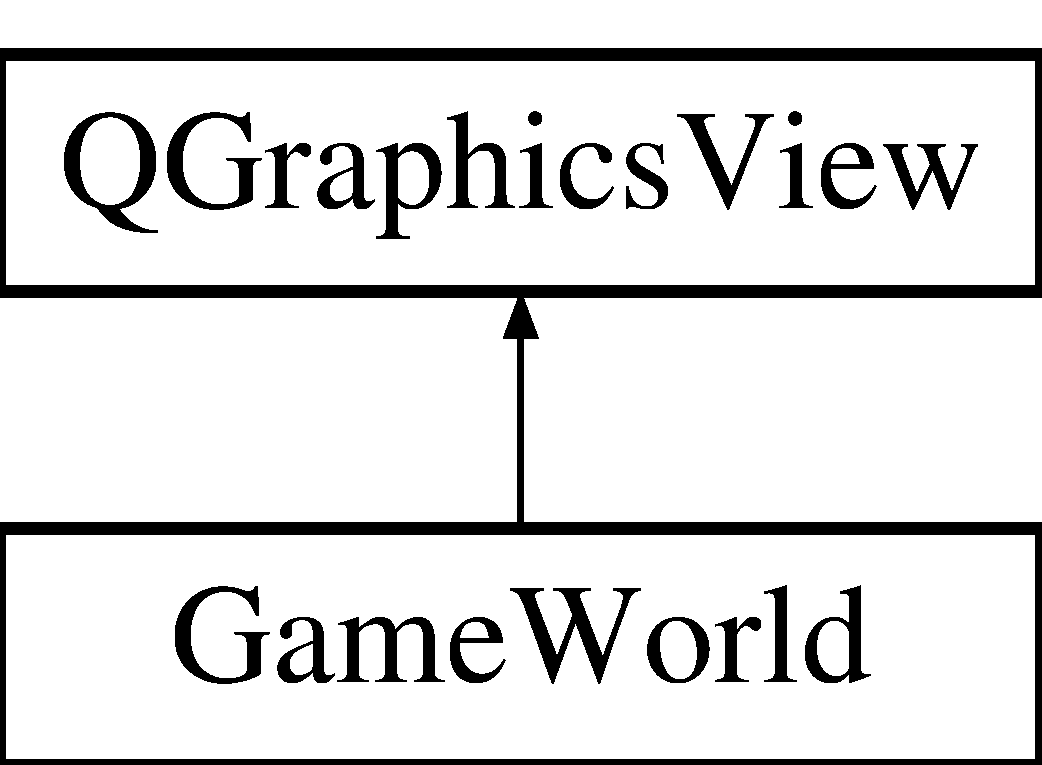
\includegraphics[height=2.000000cm]{class_game_world}
\end{center}
\end{figure}
\subsection*{Public Slots}
\begin{DoxyCompactItemize}
\item 
void {\bfseries playeronewins} ()\hypertarget{class_game_world_ada24b43c2a2c6d8147f2054a1e4a71c0}{}\label{class_game_world_ada24b43c2a2c6d8147f2054a1e4a71c0}

\item 
void {\bfseries playertwowins} ()\hypertarget{class_game_world_a6a0c32cf4eea04374ea6c4ec75ed3737}{}\label{class_game_world_a6a0c32cf4eea04374ea6c4ec75ed3737}

\item 
void {\bfseries rotate\+Background} ()\hypertarget{class_game_world_a4b17ac101198095db71b34cfd87b97b2}{}\label{class_game_world_a4b17ac101198095db71b34cfd87b97b2}

\item 
void {\bfseries display\+Meele} ()\hypertarget{class_game_world_a0b7431a3b73fbbf9a82fa1dc4bf66044}{}\label{class_game_world_a0b7431a3b73fbbf9a82fa1dc4bf66044}

\item 
void {\bfseries hide\+Meele} ()\hypertarget{class_game_world_a4933e2019efbb8f0eaab67c207ed88ae}{}\label{class_game_world_a4933e2019efbb8f0eaab67c207ed88ae}

\end{DoxyCompactItemize}
\subsection*{Signals}
\begin{DoxyCompactItemize}
\item 
void {\bfseries player\+One\+Wins\+Signal} ()\hypertarget{class_game_world_a0fbfa50d5f60312808f9e274e0f920d5}{}\label{class_game_world_a0fbfa50d5f60312808f9e274e0f920d5}

\item 
void {\bfseries player\+Two\+Wins\+Signal} ()\hypertarget{class_game_world_a7b4e0c5e973e19449250249036c98b58}{}\label{class_game_world_a7b4e0c5e973e19449250249036c98b58}

\end{DoxyCompactItemize}
\subsection*{Public Member Functions}
\begin{DoxyCompactItemize}
\item 
\hyperlink{class_game_world_a4917d80cbe417b0dc1d9023499d83f72}{Game\+World} (\hyperlink{class_sound_player}{Sound\+Player} $\ast$soundplayer)\hypertarget{class_game_world_a4917d80cbe417b0dc1d9023499d83f72}{}\label{class_game_world_a4917d80cbe417b0dc1d9023499d83f72}

\begin{DoxyCompactList}\small\item\em \hyperlink{class_game_world}{Game\+World} Constructor. \end{DoxyCompactList}\item 
void {\bfseries set\+Game\+World\+Size} (int value)\hypertarget{class_game_world_a2a8abffdaba4eee013e9b9d90e33a1ab}{}\label{class_game_world_a2a8abffdaba4eee013e9b9d90e33a1ab}

\item 
void {\bfseries pause} ()\hypertarget{class_game_world_a16bb1b2b833157573cb2a5e7de7a9ea8}{}\label{class_game_world_a16bb1b2b833157573cb2a5e7de7a9ea8}

\item 
void {\bfseries resume} ()\hypertarget{class_game_world_abac3f51224b0a62f23312534d3c642e5}{}\label{class_game_world_abac3f51224b0a62f23312534d3c642e5}

\end{DoxyCompactItemize}
\subsection*{Public Attributes}
\begin{DoxyCompactItemize}
\item 
\hyperlink{class_terrain}{Terrain} $\ast$ {\bfseries terrain}\hypertarget{class_game_world_a97a0e2bf2693f10e7ab7481ada618191}{}\label{class_game_world_a97a0e2bf2693f10e7ab7481ada618191}

\item 
\hyperlink{class_input}{Input} $\ast$ {\bfseries input}\hypertarget{class_game_world_af51a9a6f7f2f318a7f4842bc7ddddf67}{}\label{class_game_world_af51a9a6f7f2f318a7f4842bc7ddddf67}

\item 
\hyperlink{class_gameplay_interface}{Gameplay\+Interface} $\ast$ {\bfseries scene}\hypertarget{class_game_world_a470317d29e5b698b1e08dc983d78ff50}{}\label{class_game_world_a470317d29e5b698b1e08dc983d78ff50}

\item 
Q\+Timer $\ast$ {\bfseries back\+Ground\+Rotation\+Timer}\hypertarget{class_game_world_a12fff5decf2e34382c409923ec6f4668}{}\label{class_game_world_a12fff5decf2e34382c409923ec6f4668}

\item 
Q\+Graphics\+Pixmap\+Item $\ast$ {\bfseries background}\hypertarget{class_game_world_a42c3f3a06320763c952771c93f49489d}{}\label{class_game_world_a42c3f3a06320763c952771c93f49489d}

\item 
\hyperlink{class_sound_player}{Sound\+Player} $\ast$ {\bfseries soundpointer}\hypertarget{class_game_world_a133678d6bc4754bff909f0e744923549}{}\label{class_game_world_a133678d6bc4754bff909f0e744923549}

\end{DoxyCompactItemize}


\subsection{Detailed Description}
container class for \hyperlink{class_terrain}{Terrain}, \hyperlink{class_input}{Input} and \hyperlink{class_gameplay_interface}{Gameplay\+Interface}. 

Details\+: \hyperlink{class_game_world}{Game\+World} contains classes that need to communicate with each other and enables connect() functions between them. It also contains a Q\+Timer to make the background rotate. 

The documentation for this class was generated from the following files\+:\begin{DoxyCompactItemize}
\item 
World\+War\+Jump/\+World\+War\+Jump/gameworld.\+h\item 
World\+War\+Jump/\+World\+War\+Jump/gameworld.\+cpp\end{DoxyCompactItemize}

\hypertarget{class_input}{}\section{Input Class Reference}
\label{class_input}\index{Input@{Input}}
Inheritance diagram for Input\+:\begin{figure}[H]
\begin{center}
\leavevmode
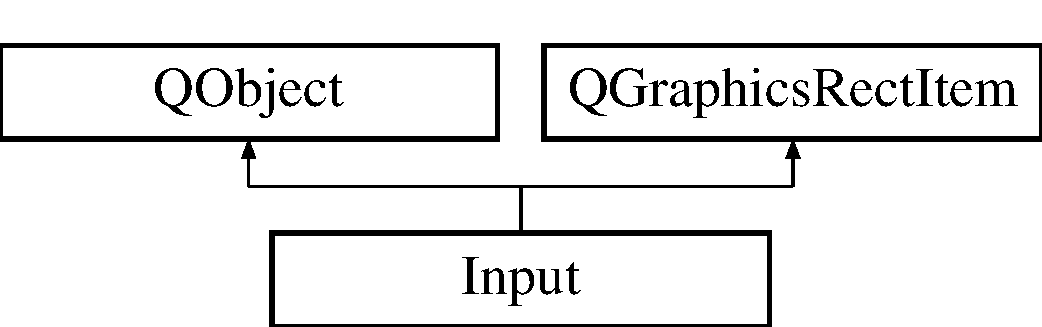
\includegraphics[height=2.000000cm]{class_input}
\end{center}
\end{figure}
\subsection*{Signals}
\begin{DoxyCompactItemize}
\item 
void {\bfseries player\+One\+Jump} ()\hypertarget{class_input_a3c56e6c2e6960014a56835cab6298d20}{}\label{class_input_a3c56e6c2e6960014a56835cab6298d20}

\item 
void {\bfseries player\+One\+Shoot} ()\hypertarget{class_input_a90a64a89b4d9804ed16c6141e9946a58}{}\label{class_input_a90a64a89b4d9804ed16c6141e9946a58}

\item 
void {\bfseries player\+Two\+Jump} ()\hypertarget{class_input_ad7689c70cb0680ed838db073af088c0a}{}\label{class_input_ad7689c70cb0680ed838db073af088c0a}

\item 
void {\bfseries player\+Two\+Shoot} ()\hypertarget{class_input_af8eba659f268b7cb19558c5a2bd40d17}{}\label{class_input_af8eba659f268b7cb19558c5a2bd40d17}

\end{DoxyCompactItemize}
\subsection*{Public Member Functions}
\begin{DoxyCompactItemize}
\item 
void {\bfseries key\+Press\+Event} (Q\+Key\+Event $\ast$k)\hypertarget{class_input_af33a8e4ba483419bd40b1c20ccc1cd7f}{}\label{class_input_af33a8e4ba483419bd40b1c20ccc1cd7f}

\end{DoxyCompactItemize}
\subsection*{Public Attributes}
\begin{DoxyCompactItemize}
\item 
Q\+Timer $\ast$ \hyperlink{class_input_a3196d6cd66f0491bc90fd7a48e2d9c9c}{refresh\+Rate\+Timer}\hypertarget{class_input_a3196d6cd66f0491bc90fd7a48e2d9c9c}{}\label{class_input_a3196d6cd66f0491bc90fd7a48e2d9c9c}

\begin{DoxyCompactList}\small\item\em Gameplay refresh rate. \end{DoxyCompactList}\end{DoxyCompactItemize}


The documentation for this class was generated from the following files\+:\begin{DoxyCompactItemize}
\item 
World\+War\+Jump/\+World\+War\+Jump/input.\+h\item 
World\+War\+Jump/\+World\+War\+Jump/input.\+cpp\end{DoxyCompactItemize}

\hypertarget{class_main_window}{}\section{Main\+Window Class Reference}
\label{class_main_window}\index{Main\+Window@{Main\+Window}}
Inheritance diagram for Main\+Window\+:\begin{figure}[H]
\begin{center}
\leavevmode
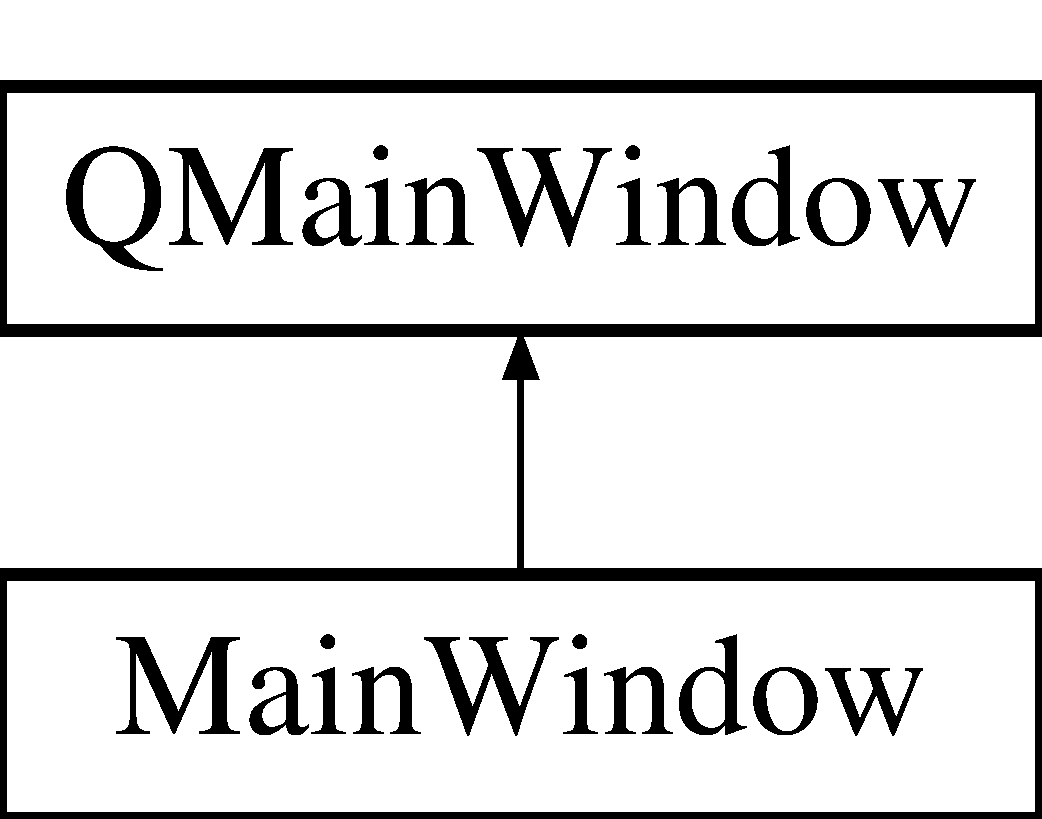
\includegraphics[height=2.000000cm]{class_main_window}
\end{center}
\end{figure}
\subsection*{Public Member Functions}
\begin{DoxyCompactItemize}
\item 
{\bfseries Main\+Window} (Q\+Widget $\ast$parent=0)\hypertarget{class_main_window_a8b244be8b7b7db1b08de2a2acb9409db}{}\label{class_main_window_a8b244be8b7b7db1b08de2a2acb9409db}

\end{DoxyCompactItemize}


The documentation for this class was generated from the following files\+:\begin{DoxyCompactItemize}
\item 
mainwindow.\+h\item 
mainwindow.\+cpp\end{DoxyCompactItemize}

\hypertarget{class_physics_calc}{}\section{Physics\+Calc Class Reference}
\label{class_physics_calc}\index{Physics\+Calc@{Physics\+Calc}}


Our own physics calculator engine and the core of the game. -\/\+Can, Tomas, Sebastian.  




{\ttfamily \#include $<$physicscalc.\+h$>$}

Inheritance diagram for Physics\+Calc\+:\begin{figure}[H]
\begin{center}
\leavevmode
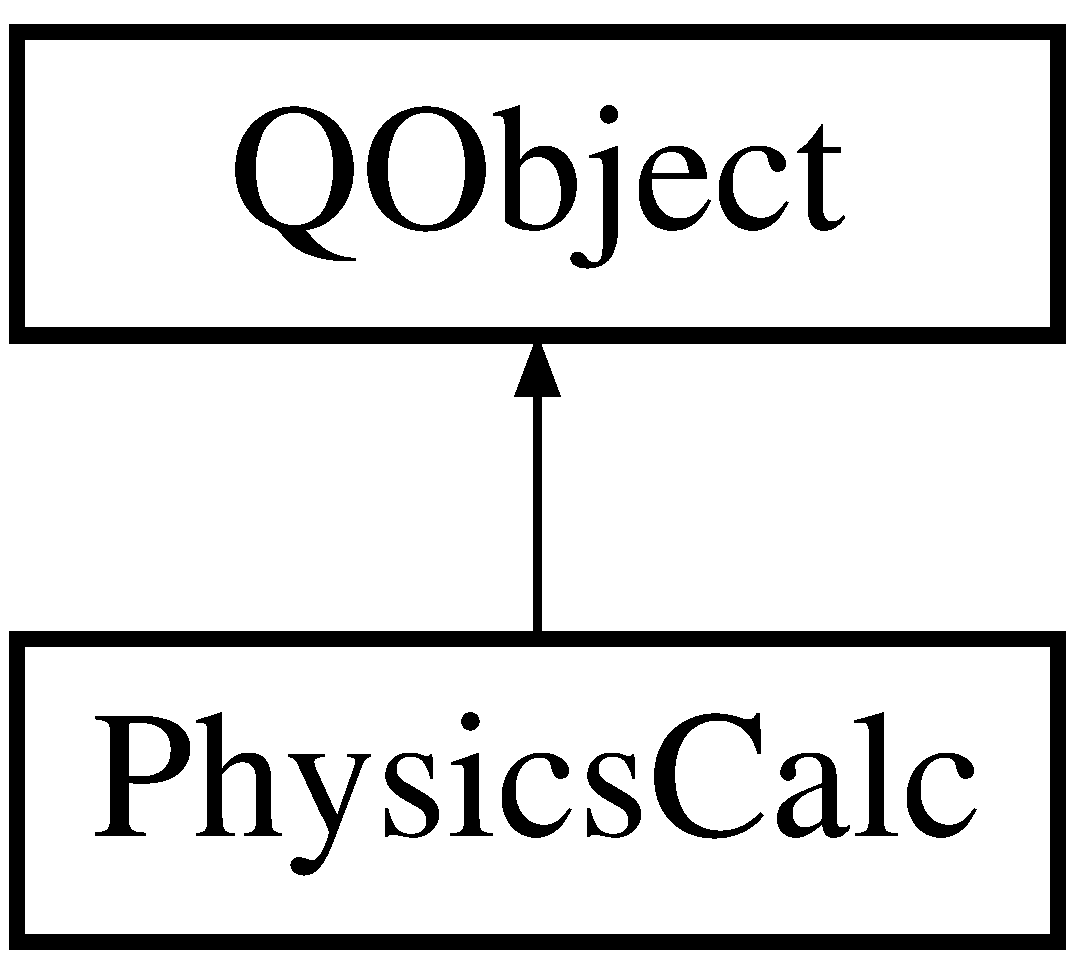
\includegraphics[height=2.000000cm]{class_physics_calc}
\end{center}
\end{figure}
\subsection*{Signals}
\begin{DoxyCompactItemize}
\item 
void {\bfseries playeronewins} ()\hypertarget{class_physics_calc_a6790d05bf566005c0f8f4fb979eeabae}{}\label{class_physics_calc_a6790d05bf566005c0f8f4fb979eeabae}

\item 
void {\bfseries playertwowins} ()\hypertarget{class_physics_calc_aee47b83ee796e172207ef43885fe1e11}{}\label{class_physics_calc_aee47b83ee796e172207ef43885fe1e11}

\item 
void {\bfseries meele\+Dmg} ()\hypertarget{class_physics_calc_a869e988d2f13341a0e0fcd22a99963aa}{}\label{class_physics_calc_a869e988d2f13341a0e0fcd22a99963aa}

\end{DoxyCompactItemize}
\subsection*{Public Member Functions}
\begin{DoxyCompactItemize}
\item 
\hyperlink{class_physics_calc_a806b2675198437e8271ab82eda0e6746}{Physics\+Calc} (\hyperlink{class_sound_player}{Sound\+Player} $\ast$soundplayer)
\begin{DoxyCompactList}\small\item\em \hyperlink{class_physics_calc_a806b2675198437e8271ab82eda0e6746}{Physics\+Calc\+::\+Physics\+Calc}. Jump\+Frame\+Limit determines how many timesteps the unit is allowed to not collide with the ground before it is able to jump again. \end{DoxyCompactList}\item 
void \hyperlink{class_physics_calc_a7ef2a6c520d3d0a815c333c1a08cb4df}{calculate\+New\+Rot\+Values} (\hyperlink{class_world_object}{World\+Object} $\ast$world\+Object)
\begin{DoxyCompactList}\small\item\em \hyperlink{class_physics_calc_a7ef2a6c520d3d0a815c333c1a08cb4df}{Physics\+Calc\+::calculate\+New\+Rot\+Values} calculates the next orientation of the given \hyperlink{class_world_object}{World\+Object} based on it\textquotesingle{}s current orientation and its current angular velocity. Angular array stores in the following order, the angle and angular velocity. Different calculations on projectiles and battleunits. The projectiles \char`\"{}head\char`\"{} is made to always point the speed vector. The Battleunits are made to slowly stand perpendicular to the gravity vector in stabilization module. The closer they get to the center, the less they are stabilized. \end{DoxyCompactList}\item 
void \hyperlink{class_physics_calc_afaa9837f796074797ea731066f09dfc3}{update\+Rot\+Values} (\hyperlink{class_world_object}{World\+Object} $\ast$world\+Object, double $\ast$angular)
\begin{DoxyCompactList}\small\item\em \hyperlink{class_physics_calc_afaa9837f796074797ea731066f09dfc3}{Physics\+Calc\+::update\+Rot\+Values} sets the objects new orientation and new angular velocity. \end{DoxyCompactList}\item 
void \hyperlink{class_physics_calc_ad1eaa72eeff1b031b08db33730d8decb}{grav\+Vec} (\hyperlink{class_world_object}{World\+Object} $\ast$world\+Object, double $\ast$gravity\+Vector)
\begin{DoxyCompactList}\small\item\em Physics\+Calc\+::gravity\+Vector gives the gravity vector effecting an objects center of mass at a certain time. First element gives the x and the second gives the y coordinate. \end{DoxyCompactList}\item 
void {\bfseries get\+Top\+Right} (\hyperlink{class_world_object}{World\+Object} $\ast$world\+Object, double $\ast$top\+Right)\hypertarget{class_physics_calc_af23c90f3041fe0b8be343ef2a35245d2}{}\label{class_physics_calc_af23c90f3041fe0b8be343ef2a35245d2}

\item 
void {\bfseries get\+Top\+Left} (\hyperlink{class_world_object}{World\+Object} $\ast$world\+Object, double $\ast$top\+Left)\hypertarget{class_physics_calc_a518d1c85e39c54bd349e02659c92b134}{}\label{class_physics_calc_a518d1c85e39c54bd349e02659c92b134}

\item 
void {\bfseries get\+Bottom\+Right} (\hyperlink{class_world_object}{World\+Object} $\ast$world\+Object, double $\ast$bottom\+Right)\hypertarget{class_physics_calc_af118ca721ecccebab2c88e53b7471320}{}\label{class_physics_calc_af118ca721ecccebab2c88e53b7471320}

\item 
void {\bfseries get\+Bottom\+Left} (\hyperlink{class_world_object}{World\+Object} $\ast$world\+Object, double $\ast$bottom\+Left)\hypertarget{class_physics_calc_a9a74039e739a8649547c6d2f8aaf7fab}{}\label{class_physics_calc_a9a74039e739a8649547c6d2f8aaf7fab}

\item 
void \hyperlink{class_physics_calc_a9bbfe3998836451d84697577c0e6195d}{get\+Impact\+Point} (\hyperlink{class_world_object}{World\+Object} $\ast$world\+Object, double $\ast$impact\+Point)
\begin{DoxyCompactList}\small\item\em \hyperlink{class_physics_calc_a9bbfe3998836451d84697577c0e6195d}{Physics\+Calc\+::get\+Impact\+Point} calculates the impact point with the cornerpoints of the given \hyperlink{class_world_object}{World\+Object}. \end{DoxyCompactList}\item 
double \hyperlink{class_physics_calc_a515dcab8395108cb37b7526adbab6ed0}{gravity\+Angle\+Difference} (double rotation, double $\ast$gravity\+Vector)
\begin{DoxyCompactList}\small\item\em \hyperlink{class_physics_calc_a515dcab8395108cb37b7526adbab6ed0}{Physics\+Calc\+::gravity\+Angle\+Difference} calculates the angle from the gravity vector to the current orientation. The positive direction is clockwise. \end{DoxyCompactList}\item 
double \hyperlink{class_physics_calc_a7e24e0769598a509705a71a0c4e8ab5d}{round\+Down} (double number\+To\+Round, int digit)
\begin{DoxyCompactList}\small\item\em \hyperlink{class_physics_calc_a7e24e0769598a509705a71a0c4e8ab5d}{Physics\+Calc\+::round\+Down} calculates the floor of a number from the given digit. \end{DoxyCompactList}\item 
void \hyperlink{class_physics_calc_a8d6de304c47a3b6be6fdfd7bacd3dcd2}{calculate\+New\+Values} (\hyperlink{class_world_object}{World\+Object} $\ast$)
\begin{DoxyCompactList}\small\item\em \hyperlink{class_physics_calc_a8d6de304c47a3b6be6fdfd7bacd3dcd2}{Physics\+Calc\+::calculate\+New\+Values} calculates the next position of the given \hyperlink{class_world_object}{World\+Object} based on it\textquotesingle{}s current position and its current speed. \end{DoxyCompactList}\item 
double \hyperlink{class_physics_calc_a5915904f1743c3a6cca6cf2b72a8d6f5}{vectors\+Absolute\+Value} (double $\ast$vector)
\begin{DoxyCompactList}\small\item\em \hyperlink{class_physics_calc_a5915904f1743c3a6cca6cf2b72a8d6f5}{Physics\+Calc\+::vectors\+Absolute\+Value} calculates the absolute value for a vector in R². \end{DoxyCompactList}\item 
void \hyperlink{class_physics_calc_aae5264bd415c1cccac4bd4628cb015a0}{velocity\+Euler\+To\+Radial\+Coordinates} (double $\ast$eul\+Input\+Position, double $\ast$input\+Vel\+Vector, double $\ast$output\+Vel\+Vector, bool euler\+To\+Radial)
\begin{DoxyCompactList}\small\item\em \hyperlink{class_physics_calc_aae5264bd415c1cccac4bd4628cb015a0}{Physics\+Calc\+::velocity\+Euler\+To\+Radial\+Coordinates} transforms the velocity of a \hyperlink{class_world_object}{World\+Object}. -\/\+Tomas. \end{DoxyCompactList}\item 
void \hyperlink{class_physics_calc_af038d3a5fe0160410456b14601a95581}{eul\+To\+Pol} (double $\ast$eul, double $\ast$pol, char type)
\begin{DoxyCompactList}\small\item\em \hyperlink{class_physics_calc_af038d3a5fe0160410456b14601a95581}{Physics\+Calc\+::eul\+To\+Pol} translates the given cartesian coordinate system to a polar coordinate system and saves them into a given output pointer. \end{DoxyCompactList}\item 
void \hyperlink{class_physics_calc_a441c3e94fe0e6eed1d96531368f50d54}{pol\+To\+Eul} (double $\ast$pol, double $\ast$eul, char type)
\begin{DoxyCompactList}\small\item\em \hyperlink{class_physics_calc_a441c3e94fe0e6eed1d96531368f50d54}{Physics\+Calc\+::pol\+To\+Eul} This function transforms polar coordinates into cartesian coordinates. \end{DoxyCompactList}\item 
Q\+Graphics\+Item $\ast$ \hyperlink{class_physics_calc_ad6d0e0e75ce2a00c15a883531f454233}{Collide\+With\+Unit} (\hyperlink{class_world_object}{World\+Object} $\ast$object)
\begin{DoxyCompactList}\small\item\em \hyperlink{class_physics_calc_ad6d0e0e75ce2a00c15a883531f454233}{Physics\+Calc\+::\+Collide\+With\+Unit} checks, if an object collides with an other object of the type \hyperlink{class_battle_unit}{Battle\+Unit} or \hyperlink{class_projectile}{Projectile} and returns that object. \end{DoxyCompactList}\item 
void \hyperlink{class_physics_calc_a75c4cfbeb112120f4ffd4839182ca25c}{hit\+Unit} (\hyperlink{class_world_object}{World\+Object} $\ast$world\+Object)
\begin{DoxyCompactList}\small\item\em \hyperlink{class_physics_calc_a75c4cfbeb112120f4ffd4839182ca25c}{Physics\+Calc\+::hit\+Unit} calculates the damage, between two colliding objects and checks one of the \hyperlink{class_world_object}{World\+Object} gets destroyed. \end{DoxyCompactList}\item 
void \hyperlink{class_physics_calc_ad30acc4f9a1111e1d611aa943aff53a3}{impuls} (\hyperlink{class_world_object}{World\+Object} $\ast$obj1, \hyperlink{class_world_object}{World\+Object} $\ast$obj2)
\begin{DoxyCompactList}\small\item\em \hyperlink{class_physics_calc_ad30acc4f9a1111e1d611aa943aff53a3}{Physics\+Calc\+::impuls} excecutes the conservation of the linear momentum for the two colliding objects obj1 and obj2. \end{DoxyCompactList}\item 
void \hyperlink{class_physics_calc_aac58c297992ee6fd388ff29c839c5693}{check\+Health} (\hyperlink{class_world_object}{World\+Object} $\ast$obj)
\begin{DoxyCompactList}\small\item\em \hyperlink{class_physics_calc_aac58c297992ee6fd388ff29c839c5693}{Physics\+Calc\+::check\+Health} checks if the given object has healtpoint lower or eqaul to zero and destroyes that unit. The unitcounter of the owining player will be decreased too. \end{DoxyCompactList}\item 
void \hyperlink{class_physics_calc_a611a891e2f01de112884cc09f25d1e33}{check\+Win\+Condition} ()\hypertarget{class_physics_calc_a611a891e2f01de112884cc09f25d1e33}{}\label{class_physics_calc_a611a891e2f01de112884cc09f25d1e33}

\begin{DoxyCompactList}\small\item\em \hyperlink{class_physics_calc_a611a891e2f01de112884cc09f25d1e33}{Physics\+Calc\+::check\+Win\+Condition} checks if one of the playes are out of units and than emit a winning signal. \end{DoxyCompactList}\item 
void \hyperlink{class_physics_calc_a22379e7ef119411e03fc8c4ba211c724}{inverse\+Speed} (\hyperlink{class_world_object}{World\+Object} $\ast$colliding1, \hyperlink{class_world_object}{World\+Object} $\ast$colliding2)
\begin{DoxyCompactList}\small\item\em \hyperlink{class_physics_calc_a22379e7ef119411e03fc8c4ba211c724}{Physics\+Calc\+::inverse\+Speed} invertes the speed of the first given Worldobject. \end{DoxyCompactList}\item 
void \hyperlink{class_physics_calc_a10a603c3fb290521b301a19600c067c4}{meele\+Damage} (\hyperlink{class_world_object}{World\+Object} $\ast$colliding1, \hyperlink{class_world_object}{World\+Object} $\ast$colliding2)
\begin{DoxyCompactList}\small\item\em \hyperlink{class_physics_calc_a10a603c3fb290521b301a19600c067c4}{Physics\+Calc\+::meele\+Damage} calculates the Meele Damage between two Objects. The unit which has a 10 values higher speed than the other deals the damage. \end{DoxyCompactList}\item 
bool \hyperlink{class_physics_calc_a8529b4af50316ef96a6bcbd029c39077}{collide\+With\+Any} (\hyperlink{class_world_object}{World\+Object} $\ast$object)
\begin{DoxyCompactList}\small\item\em \hyperlink{class_physics_calc_a8529b4af50316ef96a6bcbd029c39077}{Physics\+Calc\+::collide\+With\+Any} checks it the given object collides with either an unit or the terrain. \end{DoxyCompactList}\item 
void \hyperlink{class_physics_calc_aacab28a38556f2a29e52068f09a3a4f0}{unit\+Unit\+Collision\+Func} (\hyperlink{class_world_object}{World\+Object} $\ast$bat1, \hyperlink{class_world_object}{World\+Object} $\ast$bat2)
\begin{DoxyCompactList}\small\item\em \hyperlink{class_physics_calc_aacab28a38556f2a29e52068f09a3a4f0}{Physics\+Calc\+::unit\+Unit\+Collision\+Func} calculates the collision between two objects and chanches the speed of the units. This function is called with Battle\+Units. \end{DoxyCompactList}\item 
bool \hyperlink{class_physics_calc_a88dc6d26563c0a340cd5c4470801b419}{Collide\+With\+Terrain} (\hyperlink{class_world_object}{World\+Object} $\ast$object)
\begin{DoxyCompactList}\small\item\em Collide\+With\+Terrain checks if one touches the ground and returns a boolean argument. -\/ W\+A\+NG. \end{DoxyCompactList}\end{DoxyCompactItemize}
\subsection*{Public Attributes}
\begin{DoxyCompactItemize}
\item 
int {\bfseries Jump\+Frame\+Limit}\hypertarget{class_physics_calc_a72b7108e3e2f8cd8fb709849dbb2506c}{}\label{class_physics_calc_a72b7108e3e2f8cd8fb709849dbb2506c}

\item 
int {\bfseries bounce\+B4\+Destruction} = settings-\/$>$get\+Jump\+Count\+For\+Destruction()\hypertarget{class_physics_calc_a774c280f0c153e3a879d51f10091800a}{}\label{class_physics_calc_a774c280f0c153e3a879d51f10091800a}

\item 
\hyperlink{class_sound_player}{Sound\+Player} $\ast$ {\bfseries soundpointer}\hypertarget{class_physics_calc_aa292db7cbe605b0b7cb95a0548afcd29}{}\label{class_physics_calc_aa292db7cbe605b0b7cb95a0548afcd29}

\item 
\hyperlink{class_game_settings}{Game\+Settings} $\ast$ {\bfseries settings}\hypertarget{class_physics_calc_ace492cdc5b24e04044d0ed249917d93e}{}\label{class_physics_calc_ace492cdc5b24e04044d0ed249917d93e}

\item 
double {\bfseries gravity} = settings-\/$>$get\+Gravity()\hypertarget{class_physics_calc_ab941acb0b7803cb4dd1bc60fd3381043}{}\label{class_physics_calc_ab941acb0b7803cb4dd1bc60fd3381043}

\item 
double {\bfseries time\+Step} = settings-\/$>$get\+Time\+Step()\hypertarget{class_physics_calc_aeb23b46816202fed3cab9aa0d852f6a9}{}\label{class_physics_calc_aeb23b46816202fed3cab9aa0d852f6a9}

\end{DoxyCompactItemize}


\subsection{Detailed Description}
Our own physics calculator engine and the core of the game. -\/\+Can, Tomas, Sebastian. 

Detailed\+: It checks for collisions between units and follows a collision protocol. it checks if any player has won and emits according S\+I\+G\+N\+A\+Ls. Furthermore it calculates and triggers sounds accordingly for\+:
\begin{DoxyEnumerate}
\item Rotation of \hyperlink{class_world_object}{World\+Object} s
\item Translation of \hyperlink{class_world_object}{World\+Object} s
\item Gravity effects
\item Momentum conservation at collision
\item Recoil triggering at \hyperlink{class_battle_unit}{Battle\+Unit} shoot() 
\end{DoxyEnumerate}

\subsection{Constructor \& Destructor Documentation}
\index{Physics\+Calc@{Physics\+Calc}!Physics\+Calc@{Physics\+Calc}}
\index{Physics\+Calc@{Physics\+Calc}!Physics\+Calc@{Physics\+Calc}}
\subsubsection[{\texorpdfstring{Physics\+Calc(\+Sound\+Player $\ast$soundplayer)}{PhysicsCalc(SoundPlayer *soundplayer)}}]{\setlength{\rightskip}{0pt plus 5cm}Physics\+Calc\+::\+Physics\+Calc (
\begin{DoxyParamCaption}
\item[{{\bf Sound\+Player} $\ast$}]{soundplayer}
\end{DoxyParamCaption}
)}\hypertarget{class_physics_calc_a806b2675198437e8271ab82eda0e6746}{}\label{class_physics_calc_a806b2675198437e8271ab82eda0e6746}


\hyperlink{class_physics_calc_a806b2675198437e8271ab82eda0e6746}{Physics\+Calc\+::\+Physics\+Calc}. Jump\+Frame\+Limit determines how many timesteps the unit is allowed to not collide with the ground before it is able to jump again. 


\begin{DoxyParams}{Parameters}
{\em soundplayer} & the global soundplayer pointer \\
\hline
\end{DoxyParams}


\subsection{Member Function Documentation}
\index{Physics\+Calc@{Physics\+Calc}!calculate\+New\+Rot\+Values@{calculate\+New\+Rot\+Values}}
\index{calculate\+New\+Rot\+Values@{calculate\+New\+Rot\+Values}!Physics\+Calc@{Physics\+Calc}}
\subsubsection[{\texorpdfstring{calculate\+New\+Rot\+Values(\+World\+Object $\ast$world\+Object)}{calculateNewRotValues(WorldObject *worldObject)}}]{\setlength{\rightskip}{0pt plus 5cm}void Physics\+Calc\+::calculate\+New\+Rot\+Values (
\begin{DoxyParamCaption}
\item[{{\bf World\+Object} $\ast$}]{world\+Object}
\end{DoxyParamCaption}
)}\hypertarget{class_physics_calc_a7ef2a6c520d3d0a815c333c1a08cb4df}{}\label{class_physics_calc_a7ef2a6c520d3d0a815c333c1a08cb4df}


\hyperlink{class_physics_calc_a7ef2a6c520d3d0a815c333c1a08cb4df}{Physics\+Calc\+::calculate\+New\+Rot\+Values} calculates the next orientation of the given \hyperlink{class_world_object}{World\+Object} based on it\textquotesingle{}s current orientation and its current angular velocity. Angular array stores in the following order, the angle and angular velocity. Different calculations on projectiles and battleunits. The projectiles \char`\"{}head\char`\"{} is made to always point the speed vector. The Battleunits are made to slowly stand perpendicular to the gravity vector in stabilization module. The closer they get to the center, the less they are stabilized. 


\begin{DoxyParams}{Parameters}
{\em world\+Object} & the worldobject to be calculated \\
\hline
\end{DoxyParams}
The stabilization module only activates when the object is close to the ground -\/\+Can \index{Physics\+Calc@{Physics\+Calc}!calculate\+New\+Values@{calculate\+New\+Values}}
\index{calculate\+New\+Values@{calculate\+New\+Values}!Physics\+Calc@{Physics\+Calc}}
\subsubsection[{\texorpdfstring{calculate\+New\+Values(\+World\+Object $\ast$)}{calculateNewValues(WorldObject *)}}]{\setlength{\rightskip}{0pt plus 5cm}void Physics\+Calc\+::calculate\+New\+Values (
\begin{DoxyParamCaption}
\item[{{\bf World\+Object} $\ast$}]{world\+Object}
\end{DoxyParamCaption}
)}\hypertarget{class_physics_calc_a8d6de304c47a3b6be6fdfd7bacd3dcd2}{}\label{class_physics_calc_a8d6de304c47a3b6be6fdfd7bacd3dcd2}


\hyperlink{class_physics_calc_a8d6de304c47a3b6be6fdfd7bacd3dcd2}{Physics\+Calc\+::calculate\+New\+Values} calculates the next position of the given \hyperlink{class_world_object}{World\+Object} based on it\textquotesingle{}s current position and its current speed. 

When the \hyperlink{class_world_object}{World\+Object} moves below the ground (collision) the movement speed of the \hyperlink{class_world_object}{World\+Object} in radial direction is set in the direction of the center. Then it sets the object\textquotesingle{}s new position and new speed. -\/\+Tomas


\begin{DoxyParams}{Parameters}
{\em world\+Object} & the \hyperlink{class_world_object}{World\+Object} instance for which new position is to be calculated and set. If it is a \hyperlink{class_world_object}{World\+Object} of the type \hyperlink{class_projectile}{Projectile} ,then the \hyperlink{class_projectile}{Projectile} bounce counter is increased. \\
\hline
\end{DoxyParams}
\index{Physics\+Calc@{Physics\+Calc}!check\+Health@{check\+Health}}
\index{check\+Health@{check\+Health}!Physics\+Calc@{Physics\+Calc}}
\subsubsection[{\texorpdfstring{check\+Health(\+World\+Object $\ast$obj)}{checkHealth(WorldObject *obj)}}]{\setlength{\rightskip}{0pt plus 5cm}void Physics\+Calc\+::check\+Health (
\begin{DoxyParamCaption}
\item[{{\bf World\+Object} $\ast$}]{obj}
\end{DoxyParamCaption}
)}\hypertarget{class_physics_calc_aac58c297992ee6fd388ff29c839c5693}{}\label{class_physics_calc_aac58c297992ee6fd388ff29c839c5693}


\hyperlink{class_physics_calc_aac58c297992ee6fd388ff29c839c5693}{Physics\+Calc\+::check\+Health} checks if the given object has healtpoint lower or eqaul to zero and destroyes that unit. The unitcounter of the owining player will be decreased too. 


\begin{DoxyParams}{Parameters}
{\em obj} & is the \hyperlink{class_world_object}{World\+Object} whicht should be checked \\
\hline
\end{DoxyParams}
\index{Physics\+Calc@{Physics\+Calc}!collide\+With\+Any@{collide\+With\+Any}}
\index{collide\+With\+Any@{collide\+With\+Any}!Physics\+Calc@{Physics\+Calc}}
\subsubsection[{\texorpdfstring{collide\+With\+Any(\+World\+Object $\ast$object)}{collideWithAny(WorldObject *object)}}]{\setlength{\rightskip}{0pt plus 5cm}bool Physics\+Calc\+::collide\+With\+Any (
\begin{DoxyParamCaption}
\item[{{\bf World\+Object} $\ast$}]{object}
\end{DoxyParamCaption}
)}\hypertarget{class_physics_calc_a8529b4af50316ef96a6bcbd029c39077}{}\label{class_physics_calc_a8529b4af50316ef96a6bcbd029c39077}


\hyperlink{class_physics_calc_a8529b4af50316ef96a6bcbd029c39077}{Physics\+Calc\+::collide\+With\+Any} checks it the given object collides with either an unit or the terrain. 


\begin{DoxyParams}{Parameters}
{\em object} & is the object, which will checked. \\
\hline
\end{DoxyParams}
\begin{DoxyReturn}{Returns}
true if it collides, false if it do not. 
\end{DoxyReturn}
\index{Physics\+Calc@{Physics\+Calc}!Collide\+With\+Terrain@{Collide\+With\+Terrain}}
\index{Collide\+With\+Terrain@{Collide\+With\+Terrain}!Physics\+Calc@{Physics\+Calc}}
\subsubsection[{\texorpdfstring{Collide\+With\+Terrain(\+World\+Object $\ast$object)}{CollideWithTerrain(WorldObject *object)}}]{\setlength{\rightskip}{0pt plus 5cm}bool Physics\+Calc\+::\+Collide\+With\+Terrain (
\begin{DoxyParamCaption}
\item[{{\bf World\+Object} $\ast$}]{object}
\end{DoxyParamCaption}
)}\hypertarget{class_physics_calc_a88dc6d26563c0a340cd5c4470801b419}{}\label{class_physics_calc_a88dc6d26563c0a340cd5c4470801b419}


Collide\+With\+Terrain checks if one touches the ground and returns a boolean argument. -\/ W\+A\+NG. 

\hyperlink{class_physics_calc_a88dc6d26563c0a340cd5c4470801b419}{Physics\+Calc\+::\+Collide\+With\+Terrain} checks if the given object collides with the terrain and returns true or false.


\begin{DoxyParams}{Parameters}
{\em object} & is the \hyperlink{class_world_object}{World\+Object}, which will be checked. \\
\hline
\end{DoxyParams}
\begin{DoxyReturn}{Returns}
true if it collides, false if it does not. 
\end{DoxyReturn}
\index{Physics\+Calc@{Physics\+Calc}!Collide\+With\+Unit@{Collide\+With\+Unit}}
\index{Collide\+With\+Unit@{Collide\+With\+Unit}!Physics\+Calc@{Physics\+Calc}}
\subsubsection[{\texorpdfstring{Collide\+With\+Unit(\+World\+Object $\ast$object)}{CollideWithUnit(WorldObject *object)}}]{\setlength{\rightskip}{0pt plus 5cm}Q\+Graphics\+Item $\ast$ Physics\+Calc\+::\+Collide\+With\+Unit (
\begin{DoxyParamCaption}
\item[{{\bf World\+Object} $\ast$}]{object}
\end{DoxyParamCaption}
)}\hypertarget{class_physics_calc_ad6d0e0e75ce2a00c15a883531f454233}{}\label{class_physics_calc_ad6d0e0e75ce2a00c15a883531f454233}


\hyperlink{class_physics_calc_ad6d0e0e75ce2a00c15a883531f454233}{Physics\+Calc\+::\+Collide\+With\+Unit} checks, if an object collides with an other object of the type \hyperlink{class_battle_unit}{Battle\+Unit} or \hyperlink{class_projectile}{Projectile} and returns that object. 


\begin{DoxyParams}{Parameters}
{\em object} & is the object, which will be checked. \\
\hline
\end{DoxyParams}
\begin{DoxyReturn}{Returns}
is a pointer to the object, the object collides with 
\end{DoxyReturn}
\index{Physics\+Calc@{Physics\+Calc}!eul\+To\+Pol@{eul\+To\+Pol}}
\index{eul\+To\+Pol@{eul\+To\+Pol}!Physics\+Calc@{Physics\+Calc}}
\subsubsection[{\texorpdfstring{eul\+To\+Pol(double $\ast$eul, double $\ast$pol, char type)}{eulToPol(double *eul, double *pol, char type)}}]{\setlength{\rightskip}{0pt plus 5cm}void Physics\+Calc\+::eul\+To\+Pol (
\begin{DoxyParamCaption}
\item[{double $\ast$}]{eul, }
\item[{double $\ast$}]{pol, }
\item[{char}]{type}
\end{DoxyParamCaption}
)}\hypertarget{class_physics_calc_af038d3a5fe0160410456b14601a95581}{}\label{class_physics_calc_af038d3a5fe0160410456b14601a95581}


\hyperlink{class_physics_calc_af038d3a5fe0160410456b14601a95581}{Physics\+Calc\+::eul\+To\+Pol} translates the given cartesian coordinate system to a polar coordinate system and saves them into a given output pointer. 


\begin{DoxyParams}{Parameters}
{\em eul} & inputpointer in cartesian coordinates, \mbox{[}0\mbox{]} -\/$>$ x, \mbox{[}1\mbox{]} -\/$>$ y. \\
\hline
{\em pol} & outputpointer in polar coordinates, \mbox{[}0\mbox{]} -\/$>$ r, \mbox{[}1\mbox{]} -\/$>$ phi. \\
\hline
{\em type} & type of the translation, v -\/$>$ velocity, p -\/$>$ position \\
\hline
\end{DoxyParams}
\index{Physics\+Calc@{Physics\+Calc}!get\+Impact\+Point@{get\+Impact\+Point}}
\index{get\+Impact\+Point@{get\+Impact\+Point}!Physics\+Calc@{Physics\+Calc}}
\subsubsection[{\texorpdfstring{get\+Impact\+Point(\+World\+Object $\ast$world\+Object, double $\ast$impact\+Point)}{getImpactPoint(WorldObject *worldObject, double *impactPoint)}}]{\setlength{\rightskip}{0pt plus 5cm}void Physics\+Calc\+::get\+Impact\+Point (
\begin{DoxyParamCaption}
\item[{{\bf World\+Object} $\ast$}]{world\+Object, }
\item[{double $\ast$}]{impact\+Point}
\end{DoxyParamCaption}
)}\hypertarget{class_physics_calc_a9bbfe3998836451d84697577c0e6195d}{}\label{class_physics_calc_a9bbfe3998836451d84697577c0e6195d}


\hyperlink{class_physics_calc_a9bbfe3998836451d84697577c0e6195d}{Physics\+Calc\+::get\+Impact\+Point} calculates the impact point with the cornerpoints of the given \hyperlink{class_world_object}{World\+Object}. 


\begin{DoxyParams}{Parameters}
{\em world\+Object} & the object, which impact point should be calculated. \\
\hline
{\em impact\+Point} & is pointer to the array where the point will be saved. \\
\hline
\end{DoxyParams}
\index{Physics\+Calc@{Physics\+Calc}!gravity\+Angle\+Difference@{gravity\+Angle\+Difference}}
\index{gravity\+Angle\+Difference@{gravity\+Angle\+Difference}!Physics\+Calc@{Physics\+Calc}}
\subsubsection[{\texorpdfstring{gravity\+Angle\+Difference(double rotation, double $\ast$gravity\+Vector)}{gravityAngleDifference(double rotation, double *gravityVector)}}]{\setlength{\rightskip}{0pt plus 5cm}double Physics\+Calc\+::gravity\+Angle\+Difference (
\begin{DoxyParamCaption}
\item[{double}]{rotation, }
\item[{double $\ast$}]{gravity\+Vector}
\end{DoxyParamCaption}
)}\hypertarget{class_physics_calc_a515dcab8395108cb37b7526adbab6ed0}{}\label{class_physics_calc_a515dcab8395108cb37b7526adbab6ed0}


\hyperlink{class_physics_calc_a515dcab8395108cb37b7526adbab6ed0}{Physics\+Calc\+::gravity\+Angle\+Difference} calculates the angle from the gravity vector to the current orientation. The positive direction is clockwise. 


\begin{DoxyParams}{Parameters}
{\em rotation} & the rotation of the unit \\
\hline
{\em gravity\+Vector} & the gravity vector of the unit \\
\hline
\end{DoxyParams}
\begin{DoxyReturn}{Returns}
the difference between the units bottom and the gravity vector 
\end{DoxyReturn}
\index{Physics\+Calc@{Physics\+Calc}!grav\+Vec@{grav\+Vec}}
\index{grav\+Vec@{grav\+Vec}!Physics\+Calc@{Physics\+Calc}}
\subsubsection[{\texorpdfstring{grav\+Vec(\+World\+Object $\ast$world\+Object, double $\ast$gravity\+Vector)}{gravVec(WorldObject *worldObject, double *gravityVector)}}]{\setlength{\rightskip}{0pt plus 5cm}void Physics\+Calc\+::grav\+Vec (
\begin{DoxyParamCaption}
\item[{{\bf World\+Object} $\ast$}]{world\+Object, }
\item[{double $\ast$}]{gravity\+Vector}
\end{DoxyParamCaption}
)}\hypertarget{class_physics_calc_ad1eaa72eeff1b031b08db33730d8decb}{}\label{class_physics_calc_ad1eaa72eeff1b031b08db33730d8decb}


Physics\+Calc\+::gravity\+Vector gives the gravity vector effecting an objects center of mass at a certain time. First element gives the x and the second gives the y coordinate. 


\begin{DoxyParams}{Parameters}
{\em world\+Object} & \\
\hline
\end{DoxyParams}
\index{Physics\+Calc@{Physics\+Calc}!hit\+Unit@{hit\+Unit}}
\index{hit\+Unit@{hit\+Unit}!Physics\+Calc@{Physics\+Calc}}
\subsubsection[{\texorpdfstring{hit\+Unit(\+World\+Object $\ast$world\+Object)}{hitUnit(WorldObject *worldObject)}}]{\setlength{\rightskip}{0pt plus 5cm}void Physics\+Calc\+::hit\+Unit (
\begin{DoxyParamCaption}
\item[{{\bf World\+Object} $\ast$}]{world\+Object}
\end{DoxyParamCaption}
)}\hypertarget{class_physics_calc_a75c4cfbeb112120f4ffd4839182ca25c}{}\label{class_physics_calc_a75c4cfbeb112120f4ffd4839182ca25c}


\hyperlink{class_physics_calc_a75c4cfbeb112120f4ffd4839182ca25c}{Physics\+Calc\+::hit\+Unit} calculates the damage, between two colliding objects and checks one of the \hyperlink{class_world_object}{World\+Object} gets destroyed. 


\begin{DoxyParams}{Parameters}
{\em world\+Object} & is the \hyperlink{class_world_object}{World\+Object} for which the collision will be calculated. \\
\hline
\end{DoxyParams}
\index{Physics\+Calc@{Physics\+Calc}!impuls@{impuls}}
\index{impuls@{impuls}!Physics\+Calc@{Physics\+Calc}}
\subsubsection[{\texorpdfstring{impuls(\+World\+Object $\ast$obj1, World\+Object $\ast$obj2)}{impuls(WorldObject *obj1, WorldObject *obj2)}}]{\setlength{\rightskip}{0pt plus 5cm}void Physics\+Calc\+::impuls (
\begin{DoxyParamCaption}
\item[{{\bf World\+Object} $\ast$}]{obj1, }
\item[{{\bf World\+Object} $\ast$}]{obj2}
\end{DoxyParamCaption}
)}\hypertarget{class_physics_calc_ad30acc4f9a1111e1d611aa943aff53a3}{}\label{class_physics_calc_ad30acc4f9a1111e1d611aa943aff53a3}


\hyperlink{class_physics_calc_ad30acc4f9a1111e1d611aa943aff53a3}{Physics\+Calc\+::impuls} excecutes the conservation of the linear momentum for the two colliding objects obj1 and obj2. 


\begin{DoxyParams}{Parameters}
{\em obj1} & is the first object which collides. \\
\hline
{\em obj2} & is the secound object which collides. \\
\hline
\end{DoxyParams}
\index{Physics\+Calc@{Physics\+Calc}!inverse\+Speed@{inverse\+Speed}}
\index{inverse\+Speed@{inverse\+Speed}!Physics\+Calc@{Physics\+Calc}}
\subsubsection[{\texorpdfstring{inverse\+Speed(\+World\+Object $\ast$colliding1, World\+Object $\ast$colliding2)}{inverseSpeed(WorldObject *colliding1, WorldObject *colliding2)}}]{\setlength{\rightskip}{0pt plus 5cm}void Physics\+Calc\+::inverse\+Speed (
\begin{DoxyParamCaption}
\item[{{\bf World\+Object} $\ast$}]{colliding1, }
\item[{{\bf World\+Object} $\ast$}]{colliding2}
\end{DoxyParamCaption}
)}\hypertarget{class_physics_calc_a22379e7ef119411e03fc8c4ba211c724}{}\label{class_physics_calc_a22379e7ef119411e03fc8c4ba211c724}


\hyperlink{class_physics_calc_a22379e7ef119411e03fc8c4ba211c724}{Physics\+Calc\+::inverse\+Speed} invertes the speed of the first given Worldobject. 


\begin{DoxyParams}{Parameters}
{\em colliding1} & is the first \hyperlink{class_world_object}{World\+Object} which speed gets inverted. \\
\hline
{\em colliding2} & is the secound \hyperlink{class_world_object}{World\+Object}, which speed remains unchanged. \\
\hline
\end{DoxyParams}
\index{Physics\+Calc@{Physics\+Calc}!meele\+Damage@{meele\+Damage}}
\index{meele\+Damage@{meele\+Damage}!Physics\+Calc@{Physics\+Calc}}
\subsubsection[{\texorpdfstring{meele\+Damage(\+World\+Object $\ast$colliding1, World\+Object $\ast$colliding2)}{meeleDamage(WorldObject *colliding1, WorldObject *colliding2)}}]{\setlength{\rightskip}{0pt plus 5cm}void Physics\+Calc\+::meele\+Damage (
\begin{DoxyParamCaption}
\item[{{\bf World\+Object} $\ast$}]{colliding1, }
\item[{{\bf World\+Object} $\ast$}]{colliding2}
\end{DoxyParamCaption}
)}\hypertarget{class_physics_calc_a10a603c3fb290521b301a19600c067c4}{}\label{class_physics_calc_a10a603c3fb290521b301a19600c067c4}


\hyperlink{class_physics_calc_a10a603c3fb290521b301a19600c067c4}{Physics\+Calc\+::meele\+Damage} calculates the Meele Damage between two Objects. The unit which has a 10 values higher speed than the other deals the damage. 


\begin{DoxyParams}{Parameters}
{\em colliding1} & is the first colliding object. \\
\hline
{\em colliding2} & is the secound colliding object. \\
\hline
\end{DoxyParams}
\index{Physics\+Calc@{Physics\+Calc}!pol\+To\+Eul@{pol\+To\+Eul}}
\index{pol\+To\+Eul@{pol\+To\+Eul}!Physics\+Calc@{Physics\+Calc}}
\subsubsection[{\texorpdfstring{pol\+To\+Eul(double $\ast$pol, double $\ast$eul, char type)}{polToEul(double *pol, double *eul, char type)}}]{\setlength{\rightskip}{0pt plus 5cm}void Physics\+Calc\+::pol\+To\+Eul (
\begin{DoxyParamCaption}
\item[{double $\ast$}]{pol, }
\item[{double $\ast$}]{eul, }
\item[{char}]{type}
\end{DoxyParamCaption}
)}\hypertarget{class_physics_calc_a441c3e94fe0e6eed1d96531368f50d54}{}\label{class_physics_calc_a441c3e94fe0e6eed1d96531368f50d54}


\hyperlink{class_physics_calc_a441c3e94fe0e6eed1d96531368f50d54}{Physics\+Calc\+::pol\+To\+Eul} This function transforms polar coordinates into cartesian coordinates. 


\begin{DoxyParams}{Parameters}
{\em pol} & is the inputpointer for polar coordinates, \mbox{[}0\mbox{]} -\/$>$ x, \mbox{[}1\mbox{]} -\/$>$ y. \\
\hline
{\em eul} & is the outputpointer for the cartesian coordinates, \mbox{[}0\mbox{]} -\/$>$ r, \mbox{[}1\mbox{]} -\/$>$ phi. \\
\hline
{\em type} & type of the translation, v -\/$>$ velocity, p -\/$>$ position. \\
\hline
\end{DoxyParams}
\index{Physics\+Calc@{Physics\+Calc}!round\+Down@{round\+Down}}
\index{round\+Down@{round\+Down}!Physics\+Calc@{Physics\+Calc}}
\subsubsection[{\texorpdfstring{round\+Down(double number\+To\+Round, int digit)}{roundDown(double numberToRound, int digit)}}]{\setlength{\rightskip}{0pt plus 5cm}double Physics\+Calc\+::round\+Down (
\begin{DoxyParamCaption}
\item[{double}]{number\+To\+Round, }
\item[{int}]{digit}
\end{DoxyParamCaption}
)}\hypertarget{class_physics_calc_a7e24e0769598a509705a71a0c4e8ab5d}{}\label{class_physics_calc_a7e24e0769598a509705a71a0c4e8ab5d}


\hyperlink{class_physics_calc_a7e24e0769598a509705a71a0c4e8ab5d}{Physics\+Calc\+::round\+Down} calculates the floor of a number from the given digit. 


\begin{DoxyParams}{Parameters}
{\em number\+To\+Round} & the number to be rounded down \\
\hline
{\em digit} & the digit after which will be set to zero \\
\hline
\end{DoxyParams}
\begin{DoxyReturn}{Returns}
the rounded number 
\end{DoxyReturn}
\index{Physics\+Calc@{Physics\+Calc}!unit\+Unit\+Collision\+Func@{unit\+Unit\+Collision\+Func}}
\index{unit\+Unit\+Collision\+Func@{unit\+Unit\+Collision\+Func}!Physics\+Calc@{Physics\+Calc}}
\subsubsection[{\texorpdfstring{unit\+Unit\+Collision\+Func(\+World\+Object $\ast$bat1, World\+Object $\ast$bat2)}{unitUnitCollisionFunc(WorldObject *bat1, WorldObject *bat2)}}]{\setlength{\rightskip}{0pt plus 5cm}void Physics\+Calc\+::unit\+Unit\+Collision\+Func (
\begin{DoxyParamCaption}
\item[{{\bf World\+Object} $\ast$}]{bat1, }
\item[{{\bf World\+Object} $\ast$}]{bat2}
\end{DoxyParamCaption}
)}\hypertarget{class_physics_calc_aacab28a38556f2a29e52068f09a3a4f0}{}\label{class_physics_calc_aacab28a38556f2a29e52068f09a3a4f0}


\hyperlink{class_physics_calc_aacab28a38556f2a29e52068f09a3a4f0}{Physics\+Calc\+::unit\+Unit\+Collision\+Func} calculates the collision between two objects and chanches the speed of the units. This function is called with Battle\+Units. 


\begin{DoxyParams}{Parameters}
{\em bat1} & is the first \hyperlink{class_world_object}{World\+Object} which collides. \\
\hline
{\em bat2} & is the secound \hyperlink{class_world_object}{World\+Object} which collides. \\
\hline
\end{DoxyParams}
\index{Physics\+Calc@{Physics\+Calc}!update\+Rot\+Values@{update\+Rot\+Values}}
\index{update\+Rot\+Values@{update\+Rot\+Values}!Physics\+Calc@{Physics\+Calc}}
\subsubsection[{\texorpdfstring{update\+Rot\+Values(\+World\+Object $\ast$world\+Object, double $\ast$angular)}{updateRotValues(WorldObject *worldObject, double *angular)}}]{\setlength{\rightskip}{0pt plus 5cm}void Physics\+Calc\+::update\+Rot\+Values (
\begin{DoxyParamCaption}
\item[{{\bf World\+Object} $\ast$}]{world\+Object, }
\item[{double $\ast$}]{angular}
\end{DoxyParamCaption}
)}\hypertarget{class_physics_calc_afaa9837f796074797ea731066f09dfc3}{}\label{class_physics_calc_afaa9837f796074797ea731066f09dfc3}


\hyperlink{class_physics_calc_afaa9837f796074797ea731066f09dfc3}{Physics\+Calc\+::update\+Rot\+Values} sets the objects new orientation and new angular velocity. 


\begin{DoxyParams}{Parameters}
{\em world\+Object} & the worldobject to be updated \\
\hline
{\em angular} & the angle and angular speed to be set \\
\hline
\end{DoxyParams}
\index{Physics\+Calc@{Physics\+Calc}!vectors\+Absolute\+Value@{vectors\+Absolute\+Value}}
\index{vectors\+Absolute\+Value@{vectors\+Absolute\+Value}!Physics\+Calc@{Physics\+Calc}}
\subsubsection[{\texorpdfstring{vectors\+Absolute\+Value(double $\ast$vector)}{vectorsAbsoluteValue(double *vector)}}]{\setlength{\rightskip}{0pt plus 5cm}double Physics\+Calc\+::vectors\+Absolute\+Value (
\begin{DoxyParamCaption}
\item[{double $\ast$}]{vector}
\end{DoxyParamCaption}
)}\hypertarget{class_physics_calc_a5915904f1743c3a6cca6cf2b72a8d6f5}{}\label{class_physics_calc_a5915904f1743c3a6cca6cf2b72a8d6f5}


\hyperlink{class_physics_calc_a5915904f1743c3a6cca6cf2b72a8d6f5}{Physics\+Calc\+::vectors\+Absolute\+Value} calculates the absolute value for a vector in R². 


\begin{DoxyParams}{Parameters}
{\em vector} & \\
\hline
\end{DoxyParams}
\begin{DoxyReturn}{Returns}
absolute value of a vector in R². 
\end{DoxyReturn}
\index{Physics\+Calc@{Physics\+Calc}!velocity\+Euler\+To\+Radial\+Coordinates@{velocity\+Euler\+To\+Radial\+Coordinates}}
\index{velocity\+Euler\+To\+Radial\+Coordinates@{velocity\+Euler\+To\+Radial\+Coordinates}!Physics\+Calc@{Physics\+Calc}}
\subsubsection[{\texorpdfstring{velocity\+Euler\+To\+Radial\+Coordinates(double $\ast$eul\+Input\+Position, double $\ast$input\+Vel\+Vector, double $\ast$output\+Vel\+Vector, bool euler\+To\+Radial)}{velocityEulerToRadialCoordinates(double *eulInputPosition, double *inputVelVector, double *outputVelVector, bool eulerToRadial)}}]{\setlength{\rightskip}{0pt plus 5cm}void Physics\+Calc\+::velocity\+Euler\+To\+Radial\+Coordinates (
\begin{DoxyParamCaption}
\item[{double $\ast$}]{eul\+Input\+Position, }
\item[{double $\ast$}]{input\+Vel\+Vector, }
\item[{double $\ast$}]{output\+Vel\+Vector, }
\item[{bool}]{euler\+To\+Radial}
\end{DoxyParamCaption}
)}\hypertarget{class_physics_calc_aae5264bd415c1cccac4bd4628cb015a0}{}\label{class_physics_calc_aae5264bd415c1cccac4bd4628cb015a0}


\hyperlink{class_physics_calc_aae5264bd415c1cccac4bd4628cb015a0}{Physics\+Calc\+::velocity\+Euler\+To\+Radial\+Coordinates} transforms the velocity of a \hyperlink{class_world_object}{World\+Object}. -\/\+Tomas. 

Detailed\+: the new velocity vector is in a coordinate system which always points with the first coordinate from the center of the world through the position of the unit outwards radially. The second coordinate points facing int the same direction to the left.


\begin{DoxyParams}{Parameters}
{\em eul\+Input\+Position} & objects position to determine what direction is outward. \\
\hline
{\em eul\+Input\+Velocity} & objects velocity to transform \\
\hline
{\em radial\+Output} & first coordinate radial, second coordinate is tangential to the \hyperlink{class_terrain}{Terrain} \textquotesingle{}s circle. \\
\hline
{\em euler\+To\+Radial} & true if transforming from Euler coordinates, or false if transforming back to Euler coordinates. \\
\hline
\end{DoxyParams}


The documentation for this class was generated from the following files\+:\begin{DoxyCompactItemize}
\item 
physicscalc.\+h\item 
physicscalc.\+cpp\end{DoxyCompactItemize}

\hypertarget{class_projectile}{}\section{Projectile Class Reference}
\label{class_projectile}\index{Projectile@{Projectile}}
Inheritance diagram for Projectile\+:\begin{figure}[H]
\begin{center}
\leavevmode
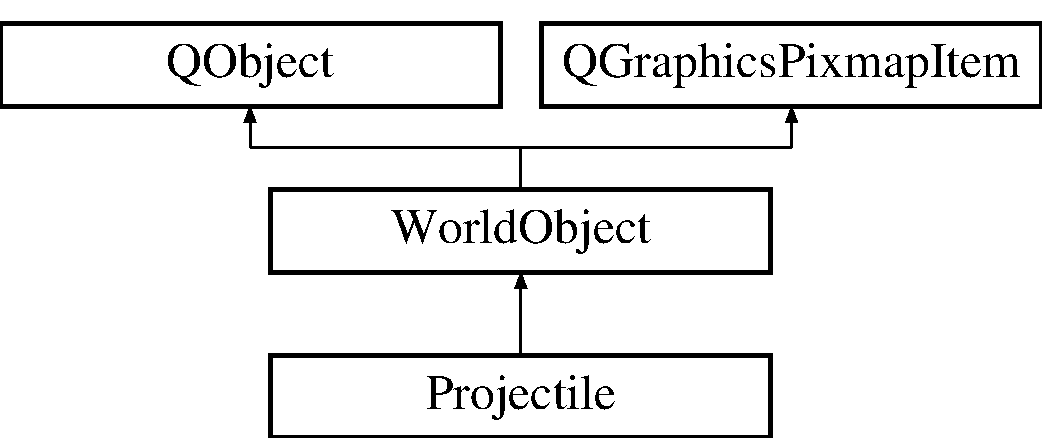
\includegraphics[height=3.000000cm]{class_projectile}
\end{center}
\end{figure}
\subsection*{Public Member Functions}
\begin{DoxyCompactItemize}
\item 
\hyperlink{class_projectile_a78d923a25fe271ac68edc1f1de95e3e8}{Projectile} (\hyperlink{class_game_world}{Game\+World} $\ast$parent\+View, \hyperlink{class_battle_unit}{Battle\+Unit} $\ast$shooting\+Unit, Projectile\+Type p, \hyperlink{class_sound_player}{Sound\+Player} $\ast$soundplayer, double $\ast$shooting\+Point)
\begin{DoxyCompactList}\small\item\em \hyperlink{class_projectile_a78d923a25fe271ac68edc1f1de95e3e8}{Projectile\+::\+Projectile} constructor. Initializes the position, the initial angle , the initial speed ,the projectile type , the weight and the damage and connects the timer It sets the picture and damage depending on the enum Player and Projectile\+Type. \end{DoxyCompactList}\item 
\hyperlink{class_projectile_a94903e021fa2edab60ba3836ca0b937d}{$\sim$\+Projectile} ()\hypertarget{class_projectile_a94903e021fa2edab60ba3836ca0b937d}{}\label{class_projectile_a94903e021fa2edab60ba3836ca0b937d}

\begin{DoxyCompactList}\small\item\em \hyperlink{class_projectile_a94903e021fa2edab60ba3836ca0b937d}{Projectile\+::$\sim$\+Projectile} This function is the destructor of the \hyperlink{class_projectile}{Projectile} class. \end{DoxyCompactList}\item 
void \hyperlink{class_projectile_a0c2d868fd9e05d3055b8f625399d7909}{recoil} (\hyperlink{class_world_object}{World\+Object} $\ast$obj1, \hyperlink{class_world_object}{World\+Object} $\ast$obj2)
\begin{DoxyCompactList}\small\item\em \hyperlink{class_projectile_a0c2d868fd9e05d3055b8f625399d7909}{Projectile\+::recoil} This function, creates a recoil on the shooting \hyperlink{class_battle_unit}{Battle\+Unit} by using the conservation of the linear momentum. \end{DoxyCompactList}\item 
void {\bfseries pol\+To\+Eul} (double $\ast$pol, double $\ast$eul, char type)\hypertarget{class_projectile_ae66148108698335706f51a19aaec764c}{}\label{class_projectile_ae66148108698335706f51a19aaec764c}

\item 
\hyperlink{class_world_object}{World\+Object} $\ast$ \hyperlink{class_projectile_aa8868e4a292212337b3d6de12e9da63a}{getshooting\+Unit} ()
\begin{DoxyCompactList}\small\item\em \hyperlink{class_projectile_aa8868e4a292212337b3d6de12e9da63a}{Projectile\+::getshooting\+Unit} This function returns the shooting\+Unit. \end{DoxyCompactList}\end{DoxyCompactItemize}
\subsection*{Additional Inherited Members}


\subsection{Constructor \& Destructor Documentation}
\index{Projectile@{Projectile}!Projectile@{Projectile}}
\index{Projectile@{Projectile}!Projectile@{Projectile}}
\subsubsection[{\texorpdfstring{Projectile(\+Game\+World $\ast$parent\+View, Battle\+Unit $\ast$shooting\+Unit, Projectile\+Type p, Sound\+Player $\ast$soundplayer, double $\ast$shooting\+Point)}{Projectile(GameWorld *parentView, BattleUnit *shootingUnit, ProjectileType p, SoundPlayer *soundplayer, double *shootingPoint)}}]{\setlength{\rightskip}{0pt plus 5cm}Projectile\+::\+Projectile (
\begin{DoxyParamCaption}
\item[{{\bf Game\+World} $\ast$}]{parent\+View, }
\item[{{\bf Battle\+Unit} $\ast$}]{shooting\+Unit, }
\item[{Projectile\+Type}]{p, }
\item[{{\bf Sound\+Player} $\ast$}]{soundplayer, }
\item[{double $\ast$}]{shooting\+Point}
\end{DoxyParamCaption}
)}\hypertarget{class_projectile_a78d923a25fe271ac68edc1f1de95e3e8}{}\label{class_projectile_a78d923a25fe271ac68edc1f1de95e3e8}


\hyperlink{class_projectile_a78d923a25fe271ac68edc1f1de95e3e8}{Projectile\+::\+Projectile} constructor. Initializes the position, the initial angle , the initial speed ,the projectile type , the weight and the damage and connects the timer It sets the picture and damage depending on the enum Player and Projectile\+Type. 


\begin{DoxyParams}{Parameters}
{\em parent\+View} & pointer to connect() the \hyperlink{class_battle_unit}{Battle\+Unit} to the player\textquotesingle{}s input and the game\textquotesingle{}s refresh rate. \\
\hline
{\em shooting\+Unit} & the battle unit shooting the projectile \\
\hline
{\em p} & the enum that gives the projectile type \\
\hline
{\em soundplayer} & the pointer to the global sound player \\
\hline
{\em shooting\+Point} & the point in scene coordinates where the projectile should spawn \\
\hline
\end{DoxyParams}


\subsection{Member Function Documentation}
\index{Projectile@{Projectile}!getshooting\+Unit@{getshooting\+Unit}}
\index{getshooting\+Unit@{getshooting\+Unit}!Projectile@{Projectile}}
\subsubsection[{\texorpdfstring{getshooting\+Unit()}{getshootingUnit()}}]{\setlength{\rightskip}{0pt plus 5cm}{\bf World\+Object} $\ast$ Projectile\+::getshooting\+Unit (
\begin{DoxyParamCaption}
{}
\end{DoxyParamCaption}
)}\hypertarget{class_projectile_aa8868e4a292212337b3d6de12e9da63a}{}\label{class_projectile_aa8868e4a292212337b3d6de12e9da63a}


\hyperlink{class_projectile_aa8868e4a292212337b3d6de12e9da63a}{Projectile\+::getshooting\+Unit} This function returns the shooting\+Unit. 

\begin{DoxyReturn}{Returns}
the shooting Unit 
\end{DoxyReturn}
\index{Projectile@{Projectile}!recoil@{recoil}}
\index{recoil@{recoil}!Projectile@{Projectile}}
\subsubsection[{\texorpdfstring{recoil(\+World\+Object $\ast$obj1, World\+Object $\ast$obj2)}{recoil(WorldObject *obj1, WorldObject *obj2)}}]{\setlength{\rightskip}{0pt plus 5cm}void Projectile\+::recoil (
\begin{DoxyParamCaption}
\item[{{\bf World\+Object} $\ast$}]{obj1, }
\item[{{\bf World\+Object} $\ast$}]{obj2}
\end{DoxyParamCaption}
)}\hypertarget{class_projectile_a0c2d868fd9e05d3055b8f625399d7909}{}\label{class_projectile_a0c2d868fd9e05d3055b8f625399d7909}


\hyperlink{class_projectile_a0c2d868fd9e05d3055b8f625399d7909}{Projectile\+::recoil} This function, creates a recoil on the shooting \hyperlink{class_battle_unit}{Battle\+Unit} by using the conservation of the linear momentum. 


\begin{DoxyParams}{Parameters}
{\em obj1} & is the Shooting \hyperlink{class_battle_unit}{Battle\+Unit} \\
\hline
{\em obj2} & is \hyperlink{class_projectile}{Projectile} \\
\hline
\end{DoxyParams}


The documentation for this class was generated from the following files\+:\begin{DoxyCompactItemize}
\item 
projectile.\+h\item 
projectile.\+cpp\end{DoxyCompactItemize}

\hypertarget{class_sound_player}{}\section{Sound\+Player Class Reference}
\label{class_sound_player}\index{Sound\+Player@{Sound\+Player}}
Inheritance diagram for Sound\+Player\+:\begin{figure}[H]
\begin{center}
\leavevmode
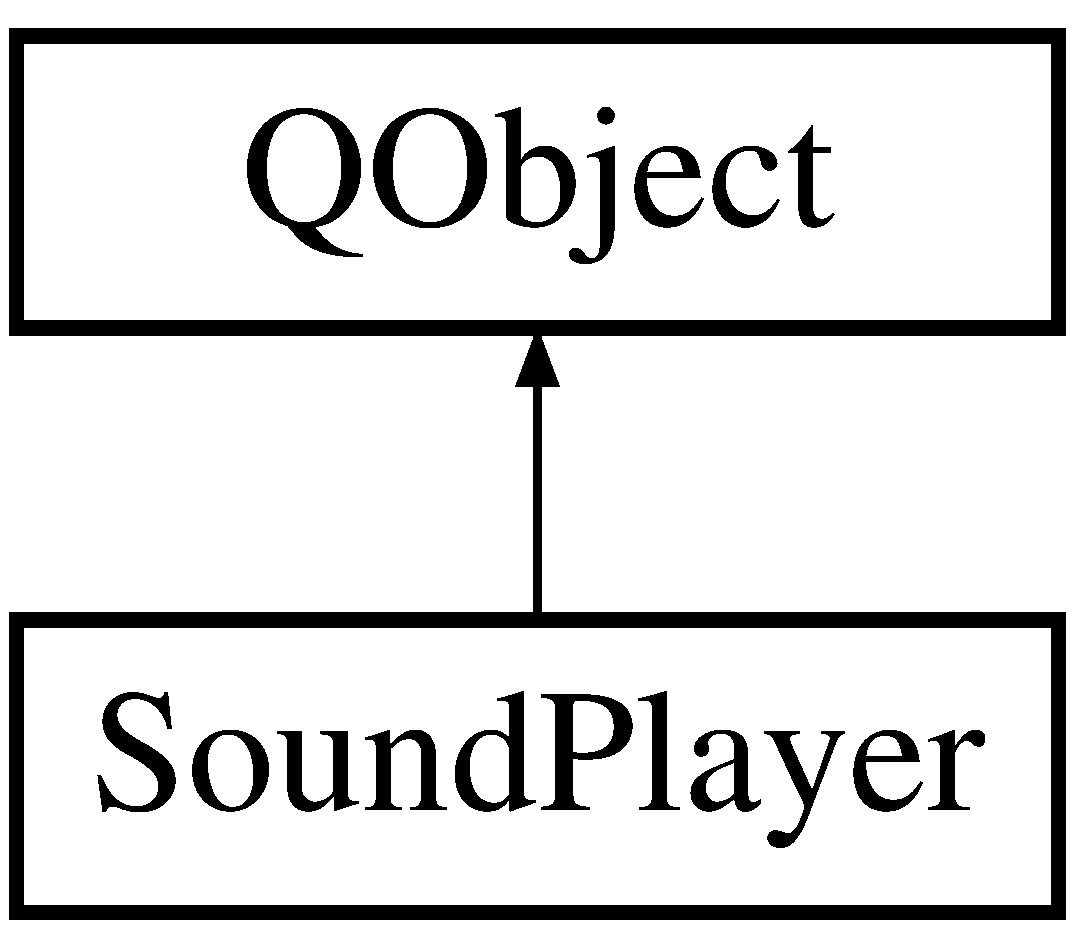
\includegraphics[height=2.000000cm]{class_sound_player}
\end{center}
\end{figure}
\subsection*{Public Member Functions}
\begin{DoxyCompactItemize}
\item 
void {\bfseries play\+Projectile\+Type\+Shoot} (int type)\hypertarget{class_sound_player_a22e1a489bbbb6cfcab3662c41f8168bc}{}\label{class_sound_player_a22e1a489bbbb6cfcab3662c41f8168bc}

\item 
void {\bfseries play\+Menu\+B\+GM} ()\hypertarget{class_sound_player_afcffc7d0a0437906496aff6ea1669193}{}\label{class_sound_player_afcffc7d0a0437906496aff6ea1669193}

\item 
void {\bfseries play\+Game\+B\+GM} ()\hypertarget{class_sound_player_a896f537cc0518edc7a724554ec35cf27}{}\label{class_sound_player_a896f537cc0518edc7a724554ec35cf27}

\item 
void {\bfseries play\+Jump} ()\hypertarget{class_sound_player_a854749ef29c5620f8b3b6355b7015d01}{}\label{class_sound_player_a854749ef29c5620f8b3b6355b7015d01}

\item 
void {\bfseries play\+Hit} ()\hypertarget{class_sound_player_a620011ab815ca67880615766518e3157}{}\label{class_sound_player_a620011ab815ca67880615766518e3157}

\end{DoxyCompactItemize}
\subsection*{Public Attributes}
\begin{DoxyCompactItemize}
\item 
Q\+Media\+Player $\ast$ {\bfseries B\+G\+Mplayer}\hypertarget{class_sound_player_a25abf7c254031e70644c8cfa1a68435b}{}\label{class_sound_player_a25abf7c254031e70644c8cfa1a68435b}

\item 
Q\+Media\+Player $\ast$ {\bfseries Jumpplayer}\hypertarget{class_sound_player_a86b10cfd0f29c18fe0a94404478d095c}{}\label{class_sound_player_a86b10cfd0f29c18fe0a94404478d095c}

\item 
Q\+Media\+Player $\ast$ {\bfseries Shoot\+Projectile\+Player}\hypertarget{class_sound_player_aab7b527b4921f87a2b0bd494cd828526}{}\label{class_sound_player_aab7b527b4921f87a2b0bd494cd828526}

\item 
Q\+Media\+Playlist $\ast$ {\bfseries Projectileplaylist}\hypertarget{class_sound_player_a14cee008aef550823022a55cea818b73}{}\label{class_sound_player_a14cee008aef550823022a55cea818b73}

\item 
Q\+Media\+Player $\ast$ {\bfseries Shoot\+Tauntplayer}\hypertarget{class_sound_player_ac5bf3fd5e40398eb110bea4453a49e55}{}\label{class_sound_player_ac5bf3fd5e40398eb110bea4453a49e55}

\item 
Q\+Media\+Playlist $\ast$ {\bfseries B\+G\+Mplaylist}\hypertarget{class_sound_player_a60736c5dd9e218a3f913c9a73883cdb6}{}\label{class_sound_player_a60736c5dd9e218a3f913c9a73883cdb6}

\item 
Q\+Media\+Player $\ast$ {\bfseries Hitplayer}\hypertarget{class_sound_player_a4ff5a304d4c03a315fbd442e92553cd0}{}\label{class_sound_player_a4ff5a304d4c03a315fbd442e92553cd0}

\item 
int {\bfseries random\+Index}\hypertarget{class_sound_player_aa3bf410aa75678aad3ab72ed50e43e02}{}\label{class_sound_player_aa3bf410aa75678aad3ab72ed50e43e02}

\end{DoxyCompactItemize}


The documentation for this class was generated from the following files\+:\begin{DoxyCompactItemize}
\item 
World\+War\+Jump/\+World\+War\+Jump/soundplayer.\+h\item 
World\+War\+Jump/\+World\+War\+Jump/soundplayer.\+cpp\end{DoxyCompactItemize}

\hypertarget{class_terrain}{}\section{Terrain Class Reference}
\label{class_terrain}\index{Terrain@{Terrain}}


\hyperlink{class_terrain}{Terrain}, the playground for our battle units in form of an inner circle. -\/ W\+A\+NG.  




{\ttfamily \#include $<$terrain.\+h$>$}

Inheritance diagram for Terrain\+:\begin{figure}[H]
\begin{center}
\leavevmode
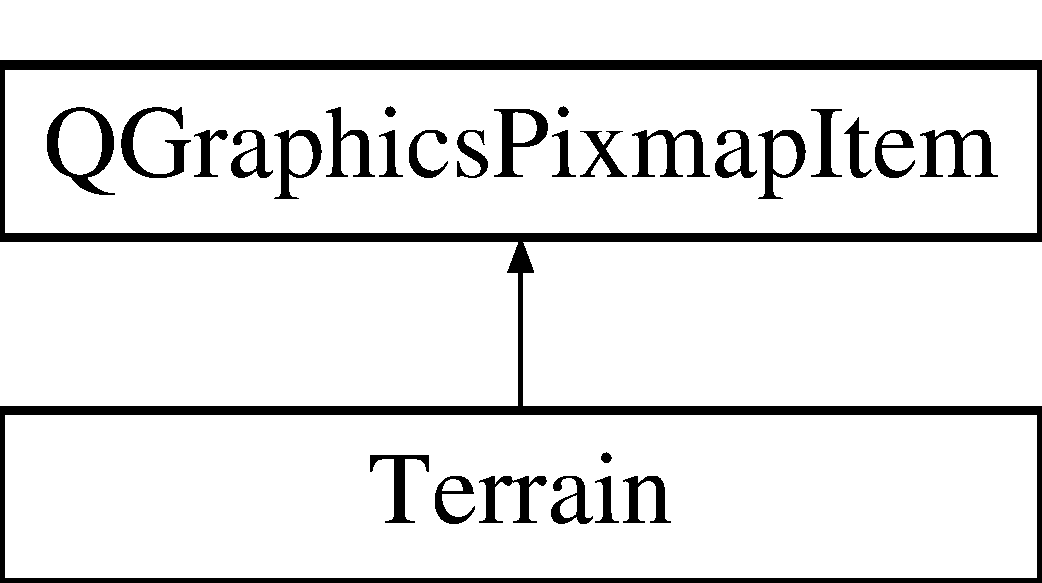
\includegraphics[height=2.000000cm]{class_terrain}
\end{center}
\end{figure}
\subsection*{Public Member Functions}
\begin{DoxyCompactItemize}
\item 
{\bfseries Terrain} (\hyperlink{class_game_settings}{Game\+Settings} $\ast$settings, \hyperlink{class_gameplay_interface}{Gameplay\+Interface} $\ast$scene)\hypertarget{class_terrain_ac711fed419262cbf10491cd392c0669b}{}\label{class_terrain_ac711fed419262cbf10491cd392c0669b}

\end{DoxyCompactItemize}


\subsection{Detailed Description}
\hyperlink{class_terrain}{Terrain}, the playground for our battle units in form of an inner circle. -\/ W\+A\+NG. 

The documentation for this class was generated from the following files\+:\begin{DoxyCompactItemize}
\item 
World\+War\+Jump/\+World\+War\+Jump/terrain.\+h\item 
World\+War\+Jump/\+World\+War\+Jump/terrain.\+cpp\end{DoxyCompactItemize}

\hypertarget{class_world_object}{}\section{World\+Object Class Reference}
\label{class_world_object}\index{World\+Object@{World\+Object}}


Basic implementation of a physical object for other classes to inheriting from. -\/ Tomas, Basti.  




{\ttfamily \#include $<$worldobject.\+h$>$}

Inheritance diagram for World\+Object\+:\begin{figure}[H]
\begin{center}
\leavevmode
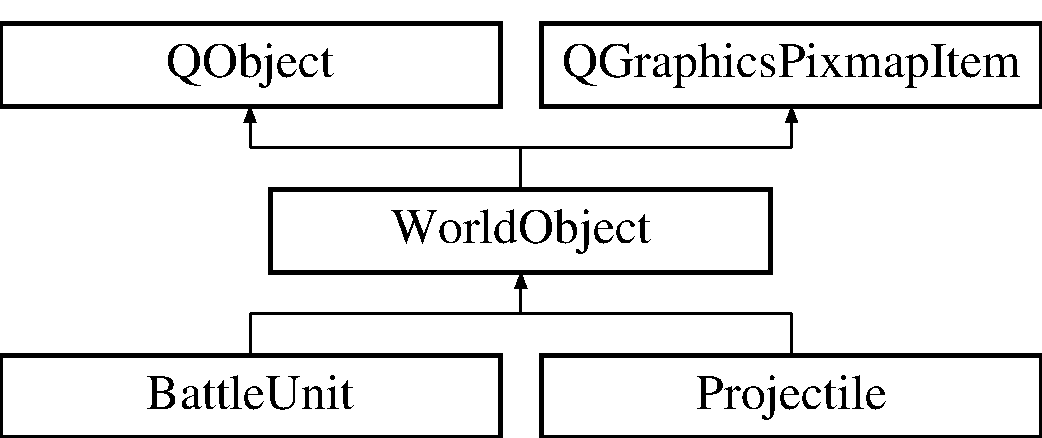
\includegraphics[height=3.000000cm]{class_world_object}
\end{center}
\end{figure}
\subsection*{Public Slots}
\begin{DoxyCompactItemize}
\item 
void \hyperlink{class_world_object_af0a581ca569f51047d53677e5d48cf30}{move} ()\hypertarget{class_world_object_af0a581ca569f51047d53677e5d48cf30}{}\label{class_world_object_af0a581ca569f51047d53677e5d48cf30}

\begin{DoxyCompactList}\small\item\em \hyperlink{class_world_object_af0a581ca569f51047d53677e5d48cf30}{World\+Object\+::move} This function is called every timestep and gets the new position and speed values for the \hyperlink{class_world_object}{World\+Object} from the physicscalc. \end{DoxyCompactList}\item 
void \hyperlink{class_world_object_a923e9f81e48251574f1b69f09ebc1c12}{jump} ()\hypertarget{class_world_object_a923e9f81e48251574f1b69f09ebc1c12}{}\label{class_world_object_a923e9f81e48251574f1b69f09ebc1c12}

\begin{DoxyCompactList}\small\item\em \hyperlink{class_world_object_a923e9f81e48251574f1b69f09ebc1c12}{World\+Object\+::jump} makes the unit jump in the direction of its head and introduces random rotation. The unit is able to jump in certain proximity to the ground, or when it is colliding with an other unit. The rotation has constant magnitude, but the direction is random. \end{DoxyCompactList}\item 
void \hyperlink{class_world_object_a5630a513886f232da0174fc992a13ad7}{hit} ()\hypertarget{class_world_object_a5630a513886f232da0174fc992a13ad7}{}\label{class_world_object_a5630a513886f232da0174fc992a13ad7}

\begin{DoxyCompactList}\small\item\em \hyperlink{class_world_object_a5630a513886f232da0174fc992a13ad7}{World\+Object\+::hit} This function is called every timestep by ervery \hyperlink{class_projectile}{Projectile} subclass to check if itself hit any \hyperlink{class_world_object}{World\+Object}. \end{DoxyCompactList}\end{DoxyCompactItemize}
\subsection*{Signals}
\begin{DoxyCompactItemize}
\item 
void {\bfseries send\+Health} (int health)\hypertarget{class_world_object_a92ca617192f2b07350e947056e67b15a}{}\label{class_world_object_a92ca617192f2b07350e947056e67b15a}

\end{DoxyCompactItemize}
\subsection*{Public Member Functions}
\begin{DoxyCompactItemize}
\item 
\hyperlink{class_world_object_a064fcf6f95ab0bcef4eaacaad35d1aee}{World\+Object} (\hyperlink{class_game_world}{Game\+World} $\ast$parent\+View, Player p, \hyperlink{class_sound_player}{Sound\+Player} $\ast$soundplayer)
\begin{DoxyCompactList}\small\item\em \hyperlink{class_world_object_a064fcf6f95ab0bcef4eaacaad35d1aee}{World\+Object\+::\+World\+Object} constructor. \end{DoxyCompactList}\item 
void \hyperlink{class_world_object_a0a4c93b5c06696aa664aae256d5378d9}{set\+Speed} (double $\ast$new\+Speed)
\begin{DoxyCompactList}\small\item\em \hyperlink{class_world_object_a0a4c93b5c06696aa664aae256d5378d9}{World\+Object\+::set\+Speed} set the speed of the unit and limit to a max speed. \end{DoxyCompactList}\item 
void {\bfseries get\+Position} (double $\ast$output\+Pointer)\hypertarget{class_world_object_a5e4d104947f9068c4d84669aad29c792}{}\label{class_world_object_a5e4d104947f9068c4d84669aad29c792}

\item 
double $\ast$ \hyperlink{class_world_object_a4a9c0e80e36b49cd7d4f574ca6351249}{get\+Speed} ()
\begin{DoxyCompactList}\small\item\em \hyperlink{class_world_object_a4a9c0e80e36b49cd7d4f574ca6351249}{World\+Object\+::get\+Speed} returns the speed of the unit. \end{DoxyCompactList}\item 
void \hyperlink{class_world_object_a0dbc4225453661d4578c7fd9eb00ab73}{set\+Orientation} (double new\+Orientation)
\begin{DoxyCompactList}\small\item\em \hyperlink{class_world_object_a0dbc4225453661d4578c7fd9eb00ab73}{World\+Object\+::set\+Orientation} set the turning angle of the unit in degrees. \end{DoxyCompactList}\item 
double \hyperlink{class_world_object_a19516f1bc3450350c42cfe467dabf4f8}{get\+Orientation} () const 
\begin{DoxyCompactList}\small\item\em \hyperlink{class_world_object_a19516f1bc3450350c42cfe467dabf4f8}{World\+Object\+::get\+Orientation} get the turning angle of the unit in degrees. \end{DoxyCompactList}\item 
void \hyperlink{class_world_object_a4fc971089870ff9db55c767694056f2f}{set\+Rot\+Vel} (double new\+Rot\+Vel)
\begin{DoxyCompactList}\small\item\em \hyperlink{class_world_object_a4fc971089870ff9db55c767694056f2f}{World\+Object\+::set\+Rot\+Vel} set the rotational velocity in degrees and limit it. \end{DoxyCompactList}\item 
double \hyperlink{class_world_object_a92c64315b40802ee97bf3cd5f16a3538}{get\+Rot\+Vel} () const 
\begin{DoxyCompactList}\small\item\em \hyperlink{class_world_object_a92c64315b40802ee97bf3cd5f16a3538}{World\+Object\+::get\+Rot\+Vel} returns the rotational velocity in degrees. \end{DoxyCompactList}\item 
void \hyperlink{class_world_object_a14befa1bd922a8c9f7134352103de942}{set\+Center\+Of\+Mass} (double $\ast$new\+Center\+Of\+Mass)
\begin{DoxyCompactList}\small\item\em \hyperlink{class_world_object_a14befa1bd922a8c9f7134352103de942}{World\+Object\+::set\+Center\+Of\+Mass} sets the position of units center of mass in scene coordinates. \end{DoxyCompactList}\item 
double $\ast$ \hyperlink{class_world_object_adec5084311ea0477db37e9bbeddeb401}{get\+Center\+Of\+Mass} ()
\begin{DoxyCompactList}\small\item\em \hyperlink{class_world_object_adec5084311ea0477db37e9bbeddeb401}{World\+Object\+::get\+Center\+Of\+Mass} gets the position of units center of mass in scene coordinates. \end{DoxyCompactList}\item 
void \hyperlink{class_world_object_aae9c6fd3df711b5e0df44ad1e6fcabab}{set\+Hit\+Counter} (int \hyperlink{class_world_object_a5630a513886f232da0174fc992a13ad7}{hit})
\begin{DoxyCompactList}\small\item\em \hyperlink{class_world_object_aae9c6fd3df711b5e0df44ad1e6fcabab}{World\+Object\+::set\+Hit\+Counter} set how many times the unit has hit the ground. \end{DoxyCompactList}\item 
int \hyperlink{class_world_object_a22888de0c352adf646e4c87584efe39c}{get\+Hit\+Counter} ()
\begin{DoxyCompactList}\small\item\em \hyperlink{class_world_object_a22888de0c352adf646e4c87584efe39c}{World\+Object\+::get\+Hit\+Counter} get how many times the unit has hit the ground. \end{DoxyCompactList}\item 
Player \hyperlink{class_world_object_ac3ff724096106165c68e3e9600032233}{get\+Player} () const 
\begin{DoxyCompactList}\small\item\em \hyperlink{class_world_object_ac3ff724096106165c68e3e9600032233}{World\+Object\+::get\+Player} returns the player controlling the unit. \end{DoxyCompactList}\item 
int \hyperlink{class_world_object_a8061ac1f99f6ed3f78d42a39cb82d0c2}{get\+Weight} ()
\begin{DoxyCompactList}\small\item\em \hyperlink{class_world_object_a8061ac1f99f6ed3f78d42a39cb82d0c2}{World\+Object\+::get\+Weight} returns the weight value of the unit. \end{DoxyCompactList}\item 
void \hyperlink{class_world_object_a39b88d87246ad4d526d6b7c54aeb7e82}{set\+Weight} (int w)
\begin{DoxyCompactList}\small\item\em \hyperlink{class_world_object_a39b88d87246ad4d526d6b7c54aeb7e82}{World\+Object\+::set\+Weight} sets the weight value of the unit. \end{DoxyCompactList}\item 
int {\bfseries get\+Healthpoints} ()\hypertarget{class_world_object_ac6f9accf985f4f67f1219ad0196a5096}{}\label{class_world_object_ac6f9accf985f4f67f1219ad0196a5096}

\item 
int {\bfseries get\+Damage} ()\hypertarget{class_world_object_ab391ed4eceba196caf01860868640f95}{}\label{class_world_object_ab391ed4eceba196caf01860868640f95}

\item 
void {\bfseries set\+Damage} (int d)\hypertarget{class_world_object_a62cc2d1b031251c40343d2b453acbd3a}{}\label{class_world_object_a62cc2d1b031251c40343d2b453acbd3a}

\item 
void \hyperlink{class_world_object_a2ad8e7e458a573830f1609f4d9d3eacf}{set\+Healthpoints} (int points)
\begin{DoxyCompactList}\small\item\em \hyperlink{class_world_object_a2ad8e7e458a573830f1609f4d9d3eacf}{World\+Object\+::set\+Healthpoints} This function sets the Healthpoints and emit a signal with the healthpoints to the healthpointsbar. \end{DoxyCompactList}\item 
void {\bfseries set\+Projectile} (int proj)\hypertarget{class_world_object_a58f877e00d7a0a05af52939e5e07c441}{}\label{class_world_object_a58f877e00d7a0a05af52939e5e07c441}

\item 
int {\bfseries get\+Projectile} ()\hypertarget{class_world_object_ae5736660e64943d305f1a400bd8f0173}{}\label{class_world_object_ae5736660e64943d305f1a400bd8f0173}

\item 
char \hyperlink{class_world_object_a4899b4a491e10707af9df49c6e6b4323}{get\+Char} ()
\begin{DoxyCompactList}\small\item\em \hyperlink{class_world_object_a4899b4a491e10707af9df49c6e6b4323}{World\+Object\+::get\+Char} returns the character indicating the unit type. If it is a battle unit, the character is \textquotesingle{}b\textquotesingle{} If it is a projectile, the character is \textquotesingle{}p\textquotesingle{} If it is neither, the character is \textquotesingle{}o\textquotesingle{}. \end{DoxyCompactList}\item 
bool \hyperlink{class_world_object_ae31450bcd5b77c1dbed862cb55ea6694}{get\+Bounced} () const 
\begin{DoxyCompactList}\small\item\em \hyperlink{class_world_object_ae31450bcd5b77c1dbed862cb55ea6694}{World\+Object\+::get\+Bounced} returns if the object has bounced before. \end{DoxyCompactList}\item 
void \hyperlink{class_world_object_a10f95129b8b184c880412181552f2208}{set\+Bounced} (bool value)
\begin{DoxyCompactList}\small\item\em \hyperlink{class_world_object_a10f95129b8b184c880412181552f2208}{World\+Object\+::set\+Bounced} sets if the object has bounced before. \end{DoxyCompactList}\item 
bool {\bfseries get\+Firstcollide} () const \hypertarget{class_world_object_a34d76ee6f6856829c59793491cab8d45}{}\label{class_world_object_a34d76ee6f6856829c59793491cab8d45}

\item 
void {\bfseries set\+Firstcollide} (bool col)\hypertarget{class_world_object_aa583750fa6789ca354abb88129b3bc2c}{}\label{class_world_object_aa583750fa6789ca354abb88129b3bc2c}

\end{DoxyCompactItemize}
\subsection*{Public Attributes}
\begin{DoxyCompactItemize}
\item 
\hyperlink{class_sound_player}{Sound\+Player} $\ast$ {\bfseries soundpointer}\hypertarget{class_world_object_aa42e809573507ad4b6a72b67521f004e}{}\label{class_world_object_aa42e809573507ad4b6a72b67521f004e}

\item 
\hyperlink{class_game_world}{Game\+World} $\ast$ {\bfseries parent\+View}\hypertarget{class_world_object_a0d420f146459b4776aab6c177847a717}{}\label{class_world_object_a0d420f146459b4776aab6c177847a717}

\item 
bool {\bfseries collided\+Before}\hypertarget{class_world_object_aa9eb87ca75a3c0147a20e214898306e2}{}\label{class_world_object_aa9eb87ca75a3c0147a20e214898306e2}

\item 
bool {\bfseries ok\+To\+Jump}\hypertarget{class_world_object_ae8ec648eb0fff181a1f99474863d2768}{}\label{class_world_object_ae8ec648eb0fff181a1f99474863d2768}

\item 
int {\bfseries jump\+Counter}\hypertarget{class_world_object_aaab8ba5520b5ea3d04b38cf86089f1c7}{}\label{class_world_object_aaab8ba5520b5ea3d04b38cf86089f1c7}

\item 
bool {\bfseries orientation\+Changed}\hypertarget{class_world_object_a79be554114fe33bdcf4ddaa2e9a970c5}{}\label{class_world_object_a79be554114fe33bdcf4ddaa2e9a970c5}

\item 
int {\bfseries orientation\+Change\+Count}\hypertarget{class_world_object_ab6317ef729bccfc2b06b10dc7a45a9e0}{}\label{class_world_object_ab6317ef729bccfc2b06b10dc7a45a9e0}

\end{DoxyCompactItemize}
\subsection*{Protected Attributes}
\begin{DoxyCompactItemize}
\item 
Player {\bfseries p}\hypertarget{class_world_object_ad976169e7d76aaee0a913852fe861787}{}\label{class_world_object_ad976169e7d76aaee0a913852fe861787}

\item 
char {\bfseries Object\+Type}\hypertarget{class_world_object_a06b54b3198229f49b5ba5dcccc7710eb}{}\label{class_world_object_a06b54b3198229f49b5ba5dcccc7710eb}

\end{DoxyCompactItemize}


\subsection{Detailed Description}
Basic implementation of a physical object for other classes to inheriting from. -\/ Tomas, Basti. 

Detailed\+: functions like \hyperlink{class_world_object_af0a581ca569f51047d53677e5d48cf30}{move()}, \hyperlink{class_world_object_a923e9f81e48251574f1b69f09ebc1c12}{jump()} + basic physical attributes like speed, rot, orientation and more. 

\subsection{Constructor \& Destructor Documentation}
\index{World\+Object@{World\+Object}!World\+Object@{World\+Object}}
\index{World\+Object@{World\+Object}!World\+Object@{World\+Object}}
\subsubsection[{\texorpdfstring{World\+Object(\+Game\+World $\ast$parent\+View, Player p, Sound\+Player $\ast$soundplayer)}{WorldObject(GameWorld *parentView, Player p, SoundPlayer *soundplayer)}}]{\setlength{\rightskip}{0pt plus 5cm}World\+Object\+::\+World\+Object (
\begin{DoxyParamCaption}
\item[{{\bf Game\+World} $\ast$}]{parent\+View, }
\item[{Player}]{p, }
\item[{{\bf Sound\+Player} $\ast$}]{soundplayer}
\end{DoxyParamCaption}
)}\hypertarget{class_world_object_a064fcf6f95ab0bcef4eaacaad35d1aee}{}\label{class_world_object_a064fcf6f95ab0bcef4eaacaad35d1aee}


\hyperlink{class_world_object_a064fcf6f95ab0bcef4eaacaad35d1aee}{World\+Object\+::\+World\+Object} constructor. 


\begin{DoxyParams}{Parameters}
{\em parent\+View} & pointer to connect() the \hyperlink{class_battle_unit}{Battle\+Unit} to the player\textquotesingle{}s input and the game\textquotesingle{}s refresh rate. \\
\hline
{\em p} & the player controlling the unit \\
\hline
{\em soundplayer} & the pointer to the global sound player \\
\hline
\end{DoxyParams}


\subsection{Member Function Documentation}
\index{World\+Object@{World\+Object}!get\+Bounced@{get\+Bounced}}
\index{get\+Bounced@{get\+Bounced}!World\+Object@{World\+Object}}
\subsubsection[{\texorpdfstring{get\+Bounced() const }{getBounced() const }}]{\setlength{\rightskip}{0pt plus 5cm}bool World\+Object\+::get\+Bounced (
\begin{DoxyParamCaption}
{}
\end{DoxyParamCaption}
) const}\hypertarget{class_world_object_ae31450bcd5b77c1dbed862cb55ea6694}{}\label{class_world_object_ae31450bcd5b77c1dbed862cb55ea6694}


\hyperlink{class_world_object_ae31450bcd5b77c1dbed862cb55ea6694}{World\+Object\+::get\+Bounced} returns if the object has bounced before. 

\begin{DoxyReturn}{Returns}
if the object has bounced before 
\end{DoxyReturn}
\index{World\+Object@{World\+Object}!get\+Center\+Of\+Mass@{get\+Center\+Of\+Mass}}
\index{get\+Center\+Of\+Mass@{get\+Center\+Of\+Mass}!World\+Object@{World\+Object}}
\subsubsection[{\texorpdfstring{get\+Center\+Of\+Mass()}{getCenterOfMass()}}]{\setlength{\rightskip}{0pt plus 5cm}double $\ast$ World\+Object\+::get\+Center\+Of\+Mass (
\begin{DoxyParamCaption}
{}
\end{DoxyParamCaption}
)}\hypertarget{class_world_object_adec5084311ea0477db37e9bbeddeb401}{}\label{class_world_object_adec5084311ea0477db37e9bbeddeb401}


\hyperlink{class_world_object_adec5084311ea0477db37e9bbeddeb401}{World\+Object\+::get\+Center\+Of\+Mass} gets the position of units center of mass in scene coordinates. 

\begin{DoxyReturn}{Returns}
the center of mass position 
\end{DoxyReturn}
\index{World\+Object@{World\+Object}!get\+Char@{get\+Char}}
\index{get\+Char@{get\+Char}!World\+Object@{World\+Object}}
\subsubsection[{\texorpdfstring{get\+Char()}{getChar()}}]{\setlength{\rightskip}{0pt plus 5cm}char World\+Object\+::get\+Char (
\begin{DoxyParamCaption}
{}
\end{DoxyParamCaption}
)}\hypertarget{class_world_object_a4899b4a491e10707af9df49c6e6b4323}{}\label{class_world_object_a4899b4a491e10707af9df49c6e6b4323}


\hyperlink{class_world_object_a4899b4a491e10707af9df49c6e6b4323}{World\+Object\+::get\+Char} returns the character indicating the unit type. If it is a battle unit, the character is \textquotesingle{}b\textquotesingle{} If it is a projectile, the character is \textquotesingle{}p\textquotesingle{} If it is neither, the character is \textquotesingle{}o\textquotesingle{}. 

\begin{DoxyReturn}{Returns}
the units type 
\end{DoxyReturn}
\index{World\+Object@{World\+Object}!get\+Hit\+Counter@{get\+Hit\+Counter}}
\index{get\+Hit\+Counter@{get\+Hit\+Counter}!World\+Object@{World\+Object}}
\subsubsection[{\texorpdfstring{get\+Hit\+Counter()}{getHitCounter()}}]{\setlength{\rightskip}{0pt plus 5cm}int World\+Object\+::get\+Hit\+Counter (
\begin{DoxyParamCaption}
{}
\end{DoxyParamCaption}
)}\hypertarget{class_world_object_a22888de0c352adf646e4c87584efe39c}{}\label{class_world_object_a22888de0c352adf646e4c87584efe39c}


\hyperlink{class_world_object_a22888de0c352adf646e4c87584efe39c}{World\+Object\+::get\+Hit\+Counter} get how many times the unit has hit the ground. 

\begin{DoxyReturn}{Returns}
the number of collisions with ground 
\end{DoxyReturn}
\index{World\+Object@{World\+Object}!get\+Orientation@{get\+Orientation}}
\index{get\+Orientation@{get\+Orientation}!World\+Object@{World\+Object}}
\subsubsection[{\texorpdfstring{get\+Orientation() const }{getOrientation() const }}]{\setlength{\rightskip}{0pt plus 5cm}double World\+Object\+::get\+Orientation (
\begin{DoxyParamCaption}
{}
\end{DoxyParamCaption}
) const}\hypertarget{class_world_object_a19516f1bc3450350c42cfe467dabf4f8}{}\label{class_world_object_a19516f1bc3450350c42cfe467dabf4f8}


\hyperlink{class_world_object_a19516f1bc3450350c42cfe467dabf4f8}{World\+Object\+::get\+Orientation} get the turning angle of the unit in degrees. 

\begin{DoxyReturn}{Returns}
the turning angle in degrees 
\end{DoxyReturn}
\index{World\+Object@{World\+Object}!get\+Player@{get\+Player}}
\index{get\+Player@{get\+Player}!World\+Object@{World\+Object}}
\subsubsection[{\texorpdfstring{get\+Player() const }{getPlayer() const }}]{\setlength{\rightskip}{0pt plus 5cm}Player World\+Object\+::get\+Player (
\begin{DoxyParamCaption}
{}
\end{DoxyParamCaption}
) const}\hypertarget{class_world_object_ac3ff724096106165c68e3e9600032233}{}\label{class_world_object_ac3ff724096106165c68e3e9600032233}


\hyperlink{class_world_object_ac3ff724096106165c68e3e9600032233}{World\+Object\+::get\+Player} returns the player controlling the unit. 

\begin{DoxyReturn}{Returns}
the player controlling the unit 
\end{DoxyReturn}
\index{World\+Object@{World\+Object}!get\+Rot\+Vel@{get\+Rot\+Vel}}
\index{get\+Rot\+Vel@{get\+Rot\+Vel}!World\+Object@{World\+Object}}
\subsubsection[{\texorpdfstring{get\+Rot\+Vel() const }{getRotVel() const }}]{\setlength{\rightskip}{0pt plus 5cm}double World\+Object\+::get\+Rot\+Vel (
\begin{DoxyParamCaption}
{}
\end{DoxyParamCaption}
) const}\hypertarget{class_world_object_a92c64315b40802ee97bf3cd5f16a3538}{}\label{class_world_object_a92c64315b40802ee97bf3cd5f16a3538}


\hyperlink{class_world_object_a92c64315b40802ee97bf3cd5f16a3538}{World\+Object\+::get\+Rot\+Vel} returns the rotational velocity in degrees. 

\begin{DoxyReturn}{Returns}
the rotational velocity in degrees 
\end{DoxyReturn}
\index{World\+Object@{World\+Object}!get\+Speed@{get\+Speed}}
\index{get\+Speed@{get\+Speed}!World\+Object@{World\+Object}}
\subsubsection[{\texorpdfstring{get\+Speed()}{getSpeed()}}]{\setlength{\rightskip}{0pt plus 5cm}double $\ast$ World\+Object\+::get\+Speed (
\begin{DoxyParamCaption}
{}
\end{DoxyParamCaption}
)}\hypertarget{class_world_object_a4a9c0e80e36b49cd7d4f574ca6351249}{}\label{class_world_object_a4a9c0e80e36b49cd7d4f574ca6351249}


\hyperlink{class_world_object_a4a9c0e80e36b49cd7d4f574ca6351249}{World\+Object\+::get\+Speed} returns the speed of the unit. 

\begin{DoxyReturn}{Returns}
the pointer to the speed array 
\end{DoxyReturn}
\index{World\+Object@{World\+Object}!get\+Weight@{get\+Weight}}
\index{get\+Weight@{get\+Weight}!World\+Object@{World\+Object}}
\subsubsection[{\texorpdfstring{get\+Weight()}{getWeight()}}]{\setlength{\rightskip}{0pt plus 5cm}int World\+Object\+::get\+Weight (
\begin{DoxyParamCaption}
{}
\end{DoxyParamCaption}
)}\hypertarget{class_world_object_a8061ac1f99f6ed3f78d42a39cb82d0c2}{}\label{class_world_object_a8061ac1f99f6ed3f78d42a39cb82d0c2}


\hyperlink{class_world_object_a8061ac1f99f6ed3f78d42a39cb82d0c2}{World\+Object\+::get\+Weight} returns the weight value of the unit. 

\begin{DoxyReturn}{Returns}
the weight 
\end{DoxyReturn}
\index{World\+Object@{World\+Object}!set\+Bounced@{set\+Bounced}}
\index{set\+Bounced@{set\+Bounced}!World\+Object@{World\+Object}}
\subsubsection[{\texorpdfstring{set\+Bounced(bool value)}{setBounced(bool value)}}]{\setlength{\rightskip}{0pt plus 5cm}void World\+Object\+::set\+Bounced (
\begin{DoxyParamCaption}
\item[{bool}]{value}
\end{DoxyParamCaption}
)}\hypertarget{class_world_object_a10f95129b8b184c880412181552f2208}{}\label{class_world_object_a10f95129b8b184c880412181552f2208}


\hyperlink{class_world_object_a10f95129b8b184c880412181552f2208}{World\+Object\+::set\+Bounced} sets if the object has bounced before. 


\begin{DoxyParams}{Parameters}
{\em value} & the bool value indicating if the object has bounced before or not \\
\hline
\end{DoxyParams}
\index{World\+Object@{World\+Object}!set\+Center\+Of\+Mass@{set\+Center\+Of\+Mass}}
\index{set\+Center\+Of\+Mass@{set\+Center\+Of\+Mass}!World\+Object@{World\+Object}}
\subsubsection[{\texorpdfstring{set\+Center\+Of\+Mass(double $\ast$new\+Center\+Of\+Mass)}{setCenterOfMass(double *newCenterOfMass)}}]{\setlength{\rightskip}{0pt plus 5cm}void World\+Object\+::set\+Center\+Of\+Mass (
\begin{DoxyParamCaption}
\item[{double $\ast$}]{new\+Center\+Of\+Mass}
\end{DoxyParamCaption}
)}\hypertarget{class_world_object_a14befa1bd922a8c9f7134352103de942}{}\label{class_world_object_a14befa1bd922a8c9f7134352103de942}


\hyperlink{class_world_object_a14befa1bd922a8c9f7134352103de942}{World\+Object\+::set\+Center\+Of\+Mass} sets the position of units center of mass in scene coordinates. 


\begin{DoxyParams}{Parameters}
{\em new\+Center\+Of\+Mass} & the new center of mass position \\
\hline
\end{DoxyParams}
\index{World\+Object@{World\+Object}!set\+Healthpoints@{set\+Healthpoints}}
\index{set\+Healthpoints@{set\+Healthpoints}!World\+Object@{World\+Object}}
\subsubsection[{\texorpdfstring{set\+Healthpoints(int points)}{setHealthpoints(int points)}}]{\setlength{\rightskip}{0pt plus 5cm}void World\+Object\+::set\+Healthpoints (
\begin{DoxyParamCaption}
\item[{int}]{points}
\end{DoxyParamCaption}
)}\hypertarget{class_world_object_a2ad8e7e458a573830f1609f4d9d3eacf}{}\label{class_world_object_a2ad8e7e458a573830f1609f4d9d3eacf}


\hyperlink{class_world_object_a2ad8e7e458a573830f1609f4d9d3eacf}{World\+Object\+::set\+Healthpoints} This function sets the Healthpoints and emit a signal with the healthpoints to the healthpointsbar. 


\begin{DoxyParams}{Parameters}
{\em points} & are the lifepoints \\
\hline
\end{DoxyParams}
\index{World\+Object@{World\+Object}!set\+Hit\+Counter@{set\+Hit\+Counter}}
\index{set\+Hit\+Counter@{set\+Hit\+Counter}!World\+Object@{World\+Object}}
\subsubsection[{\texorpdfstring{set\+Hit\+Counter(int hit)}{setHitCounter(int hit)}}]{\setlength{\rightskip}{0pt plus 5cm}void World\+Object\+::set\+Hit\+Counter (
\begin{DoxyParamCaption}
\item[{int}]{hit}
\end{DoxyParamCaption}
)}\hypertarget{class_world_object_aae9c6fd3df711b5e0df44ad1e6fcabab}{}\label{class_world_object_aae9c6fd3df711b5e0df44ad1e6fcabab}


\hyperlink{class_world_object_aae9c6fd3df711b5e0df44ad1e6fcabab}{World\+Object\+::set\+Hit\+Counter} set how many times the unit has hit the ground. 


\begin{DoxyParams}{Parameters}
{\em hit} & the number of collisions with ground \\
\hline
\end{DoxyParams}
\index{World\+Object@{World\+Object}!set\+Orientation@{set\+Orientation}}
\index{set\+Orientation@{set\+Orientation}!World\+Object@{World\+Object}}
\subsubsection[{\texorpdfstring{set\+Orientation(double new\+Orientation)}{setOrientation(double newOrientation)}}]{\setlength{\rightskip}{0pt plus 5cm}void World\+Object\+::set\+Orientation (
\begin{DoxyParamCaption}
\item[{double}]{new\+Orientation}
\end{DoxyParamCaption}
)}\hypertarget{class_world_object_a0dbc4225453661d4578c7fd9eb00ab73}{}\label{class_world_object_a0dbc4225453661d4578c7fd9eb00ab73}


\hyperlink{class_world_object_a0dbc4225453661d4578c7fd9eb00ab73}{World\+Object\+::set\+Orientation} set the turning angle of the unit in degrees. 


\begin{DoxyParams}{Parameters}
{\em new\+Orientation} & the new angle in degrees \\
\hline
\end{DoxyParams}
\index{World\+Object@{World\+Object}!set\+Rot\+Vel@{set\+Rot\+Vel}}
\index{set\+Rot\+Vel@{set\+Rot\+Vel}!World\+Object@{World\+Object}}
\subsubsection[{\texorpdfstring{set\+Rot\+Vel(double new\+Rot\+Vel)}{setRotVel(double newRotVel)}}]{\setlength{\rightskip}{0pt plus 5cm}void World\+Object\+::set\+Rot\+Vel (
\begin{DoxyParamCaption}
\item[{double}]{new\+Rot\+Vel}
\end{DoxyParamCaption}
)}\hypertarget{class_world_object_a4fc971089870ff9db55c767694056f2f}{}\label{class_world_object_a4fc971089870ff9db55c767694056f2f}


\hyperlink{class_world_object_a4fc971089870ff9db55c767694056f2f}{World\+Object\+::set\+Rot\+Vel} set the rotational velocity in degrees and limit it. 


\begin{DoxyParams}{Parameters}
{\em new\+Rot\+Vel} & the new rotational velocity in degrees \\
\hline
\end{DoxyParams}
\index{World\+Object@{World\+Object}!set\+Speed@{set\+Speed}}
\index{set\+Speed@{set\+Speed}!World\+Object@{World\+Object}}
\subsubsection[{\texorpdfstring{set\+Speed(double $\ast$new\+Speed)}{setSpeed(double *newSpeed)}}]{\setlength{\rightskip}{0pt plus 5cm}void World\+Object\+::set\+Speed (
\begin{DoxyParamCaption}
\item[{double $\ast$}]{new\+Speed}
\end{DoxyParamCaption}
)}\hypertarget{class_world_object_a0a4c93b5c06696aa664aae256d5378d9}{}\label{class_world_object_a0a4c93b5c06696aa664aae256d5378d9}


\hyperlink{class_world_object_a0a4c93b5c06696aa664aae256d5378d9}{World\+Object\+::set\+Speed} set the speed of the unit and limit to a max speed. 


\begin{DoxyParams}{Parameters}
{\em new\+Speed} & the pointer to the new speed array \\
\hline
\end{DoxyParams}
\index{World\+Object@{World\+Object}!set\+Weight@{set\+Weight}}
\index{set\+Weight@{set\+Weight}!World\+Object@{World\+Object}}
\subsubsection[{\texorpdfstring{set\+Weight(int w)}{setWeight(int w)}}]{\setlength{\rightskip}{0pt plus 5cm}void World\+Object\+::set\+Weight (
\begin{DoxyParamCaption}
\item[{int}]{w}
\end{DoxyParamCaption}
)}\hypertarget{class_world_object_a39b88d87246ad4d526d6b7c54aeb7e82}{}\label{class_world_object_a39b88d87246ad4d526d6b7c54aeb7e82}


\hyperlink{class_world_object_a39b88d87246ad4d526d6b7c54aeb7e82}{World\+Object\+::set\+Weight} sets the weight value of the unit. 


\begin{DoxyParams}{Parameters}
{\em w} & the new weight value \\
\hline
\end{DoxyParams}


The documentation for this class was generated from the following files\+:\begin{DoxyCompactItemize}
\item 
World\+War\+Jump/\+World\+War\+Jump/worldobject.\+h\item 
World\+War\+Jump/\+World\+War\+Jump/worldobject.\+cpp\end{DoxyCompactItemize}

%--- End generated contents ---

% Index
\backmatter
\newpage
\phantomsection
\clearemptydoublepage
\addcontentsline{toc}{chapter}{Index}
\printindex

\end{document}
